% \documentclass[handout,xcolor=pdftex,dvipsnames,table]{beamer}

%\documentclass[aspectratio=169]{beamer} % WIDESCREEN
\documentclass[t]{beamer} % Aspecto 4:3

\usepackage[utf8]{inputenc}
\usepackage[T1]{fontenc}
\usepackage[english,brazil]{babel}
%\usepackage{natbib}

\usepackage{tikz}

% usando tema personalizado.
% arquivo beamerthemeUFFS.sty deve estar no mesmo diretório do .tex
\usepackage{beamerthemeUFFS}
\usepackage{ragged2e}
\usepackage{setspace}
\usepackage{animate}

\hypersetup{
    pdfstartview={Fit},
    pdftitle={Geração procedural de biomas},
 	pdfsubject={ApresentacaoDefesaTCC1},
 	pdfauthor={João Carlos Becker}
}

%%%%%%%%%%%%%%%%%%%%%%%%%%%%%%%%%%%%%%%%%%%%
 
\title{Geração procedural de biomas}
\author{João Carlos Becker} 

%\date{28 de junho de 2016}
\institute{Ciência da Computação\\
Universidade Federal da Fronteira Sul - Chapecó}

%%%%%%%%%%%%%%%%%%%%%%%%%%%%%%%%%%%%%%%%%%%%

\begin{document}

\setstretch{1} %espaçamento

\addtobeamertemplate{frametitle}{}{%
\begin{tikzpicture}[remember picture,overlay]
\node[anchor=north east,yshift=2pt] at (current page.north east) {
\includegraphics[height=1cm]{img/logo_curso}};
\end{tikzpicture}}

\setbeamertemplate{footline}{
	\color{white}
     \\
    }

\begin{frame}
	\maketitle
\end{frame}

\addtocounter{framenumber}{-1}

% Descomente as linhas abaixo se desejar colocar um sumário de todas as seções
%\begin{frame}[t]{Sumário}
%\tableofcontents
%\end{frame}
\setbeamertemplate{footline}{
    \color{black}
    \hfill \insertframenumber\,/\,\inserttotalframenumber~
}

%Utilizado para alinhar figuras
\setbeamertemplate{caption}{\raggedright\insertcaption\par}

\def\sectionname{}
\def\insertsectionnumber{}
\def\subsectionname{}
\def\insertsubsectionnumber{}

\AtBeginSection{\frame{\sectionpage}\addtocounter{framenumber}{-1}}


\AtBeginSubsection{\frame{\subsectionpage}\addtocounter{framenumber}{-1} }
\AtBeginSubsubsection{\frame{\subsubsectionpage}\addtocounter{framenumber}{-1} }


%%%%%%%%%%%%%%%%%%%%%%%%%%%%%%%%%%%%%%%%%%%%
% Inicio do documento
%%%%%%%%%%%%%%%%%%%%%%%%%%%%%%%%%%%%%%%%%%%%

\begin{frame}{Roteiro}
  \begin{itemize} \setlength\itemsep{1em}
    \item Objetivo.
    \item Perlin Noise
\end{itemize}
\end{frame}
\begin{frame}{Problemática}
    \begin{itemize} \setlength\itemsep{1em}
        \item Os jogos digitais estão cada vez melhores e exigindo mais
        complexidade para os mesmos, trazendo mais conteúdo agregado
        \item O tempo para produzir este conteúdo demanda muito esforço de trabalho.
    \end{itemize}
\end{frame}
\begin{frame}{Problemática}
    \begin{itemize} \setlength\itemsep{1em}
        \item Os jogos digitais estão cada vez melhores e exigindo mais
        complexidade para os mesmos, trazendo mais conteúdo agregado.
        \item O tempo para produzir este conteúdo demanda muito esforço de trabalho.
    \end{itemize}
\end{frame}


%\begin{frame}{Introdução}
%    
%\end{frame}

\begin{frame}{Objetivos}
    \begin{itemize}
        \item Objetivo Geral
        \begin{itemize}
            \item Este projeto tem como objetivo gerar mapas de tamanho pseudo-infinitos, com 
            relevo gerado proceduralmente usando ruído 
            de Perlin, de maneira não assistida, os mapas de altura devem representar o 
            relevo de pelo menos dois biomas arbitrários com fronteiras contínuas.
        \end{itemize}
        \item Objetivos Específicos
        \begin{itemize}
            \item Implementar malhas da superfície com tamanho pseudo-infinito;
            \item Selecionar biomas, e as características dos mesmos a ser representadas;
            \item Construir algoritmo para manipular ruído de Perlin e gerar características
                selecionadas do bioma;
            \item Gerar divisões entre biomas sobre a malha de regiões;
            \item Implementar fronteiras contínuas entre biomas;
            \item Comparar resultado com cenários de jogos.
        \end{itemize}
    \end{itemize}
\end{frame}
\chapter{Objetivos}

\section{Objetivo Geral}
Este projeto tem como objetivo gerar mapas de tamanho pseudo-infinitos, com 
relevo gerado proceduralmente usando ruído 
de Perlin, de maneira não assistida, os mapas de altura devem representar o 
relevo de pelo menos dois biomas arbitrários com fronteiras contínuas.

%Criar um método procedural para múltiplos biomas ter fronteiras contínuas

\section{Objetivo Específico}

\begin{itemize}
    \item Implementar malhas da superfície com tamanho pseudo-infinito;
    \item Selecionar biomas, e as características dos mesmos a ser representadas;
    \item Construir algoritmo para manipular ruído de Perlin e gerar características
        selecionadas do bioma;
    \item Gerar divisões entre biomas sobre a malha de regiões;
    \item Implementar fronteiras contínuas entre biomas;
    \item Comparar resultado com cenários de jogos;
    \item Comparar resultados com a natureza.
\end{itemize}


%Me parece que justificativa está na problemática
%\section{Justificativa}



%acho que preciso fazer uma seção ou capitulo apenas para a metodologia
%\section{Metodologia}
\begin{frame}{Biomas}
    \begin{itemize} \setlength\itemsep{1em}
        \item Neste trabalho biomas são características de relevo;
        \item Foram implementados cinco biomas distintos;
        \item Suas características de cor e cálculo de altura foram escolhidos arbitrariamente
        para serem distitos.
    \end{itemize}
    
%    \begin{figure}
%        \centering
%        \begin{subfigure}[b]{0.47\textwidth}
%            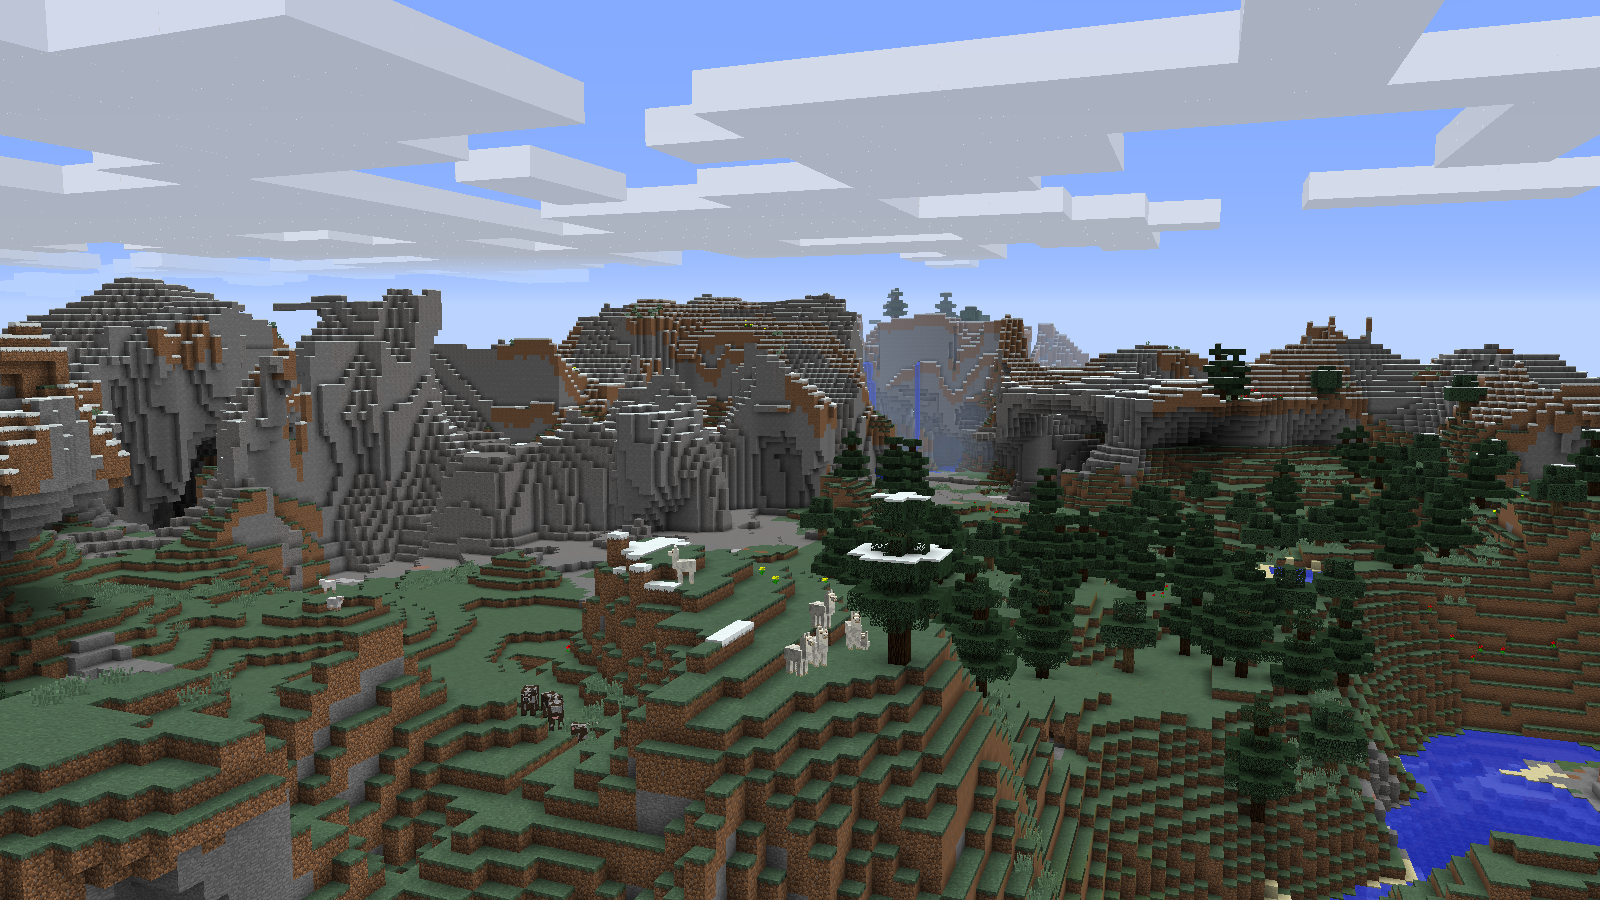
\includegraphics[width=\textwidth]{img/mineExtremeHills}
%            \caption{Bioma \textit{Extreme Hills} no minecraft}
%            \label{fig:mineExtremeHills}
%        \end{subfigure}
%        ~ %add desired spacing between images, e. g. ~, \quad, \qquad, \hfill etc. 
%          %(or a blank line to force the subfigure onto a new line)
%        \begin{subfigure}[b]{0.47\textwidth}
%            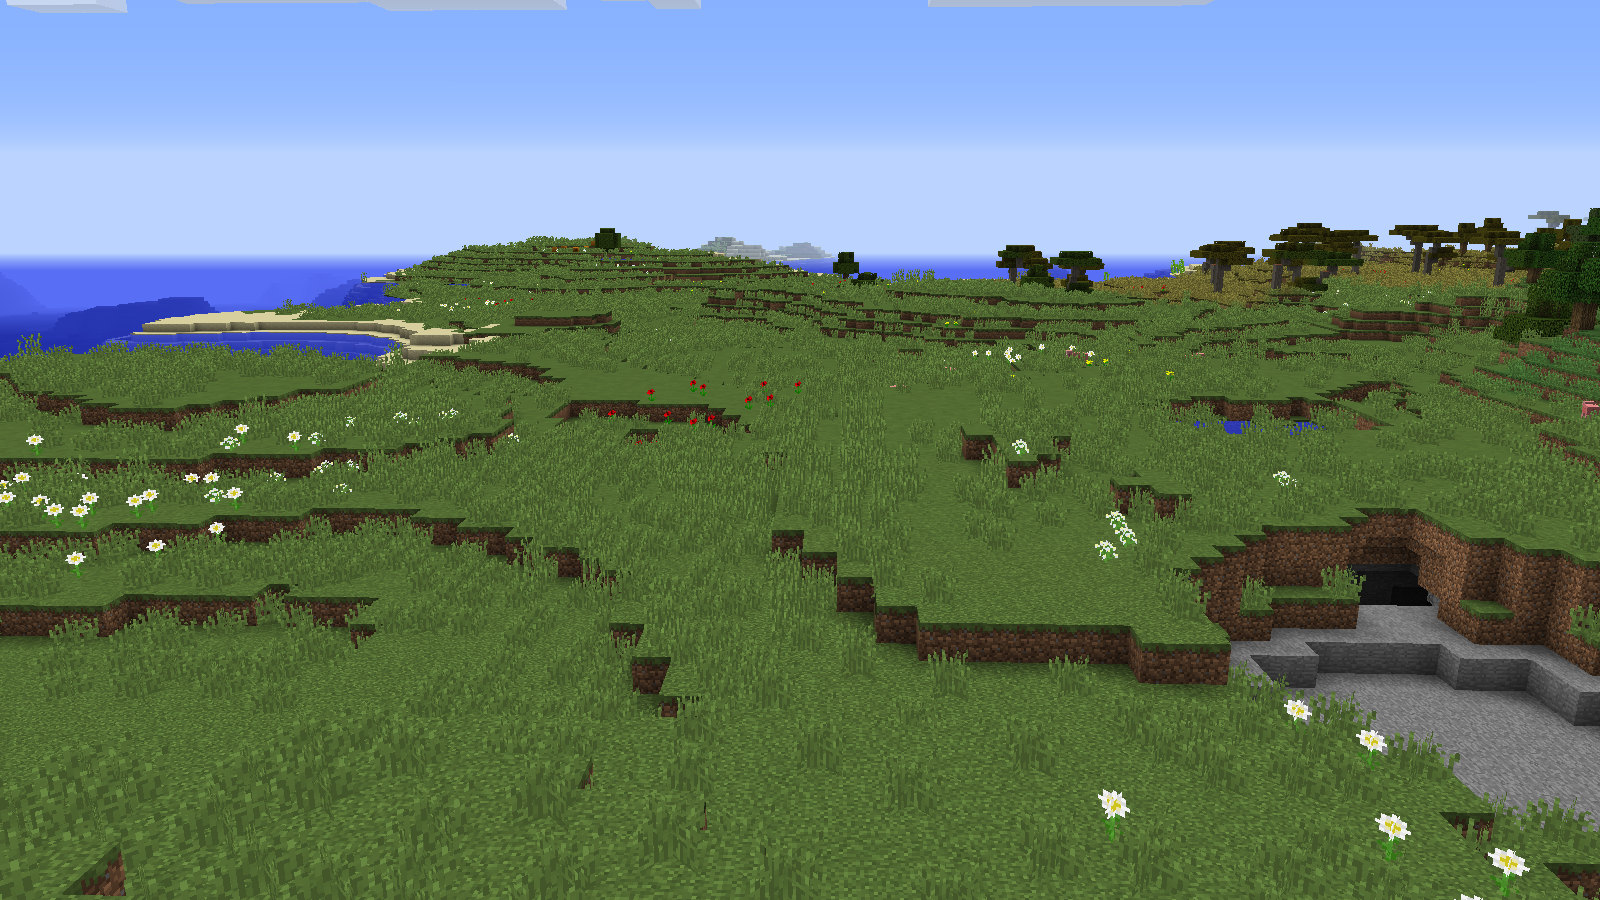
\includegraphics[width=\textwidth]{img/minePlains}
%            \caption{Bioma \textit{Plains} no minecraft}
%            \label{fig:minePlains}
%        \end{subfigure}
%        ~ %add desired spacing between images, e. g. ~, \quad, \qquad, \hfill etc. 
%        %(or a blank line to force the subfigure onto a new line)
%        \caption{Exemplo de Biomas no minecraft}
%        \label{fig:mineBiomes}
%    \end{figure}
    
    
\end{frame}

\begin{frame}{Biomas}
    \begin{figure}[H]
        \centering
        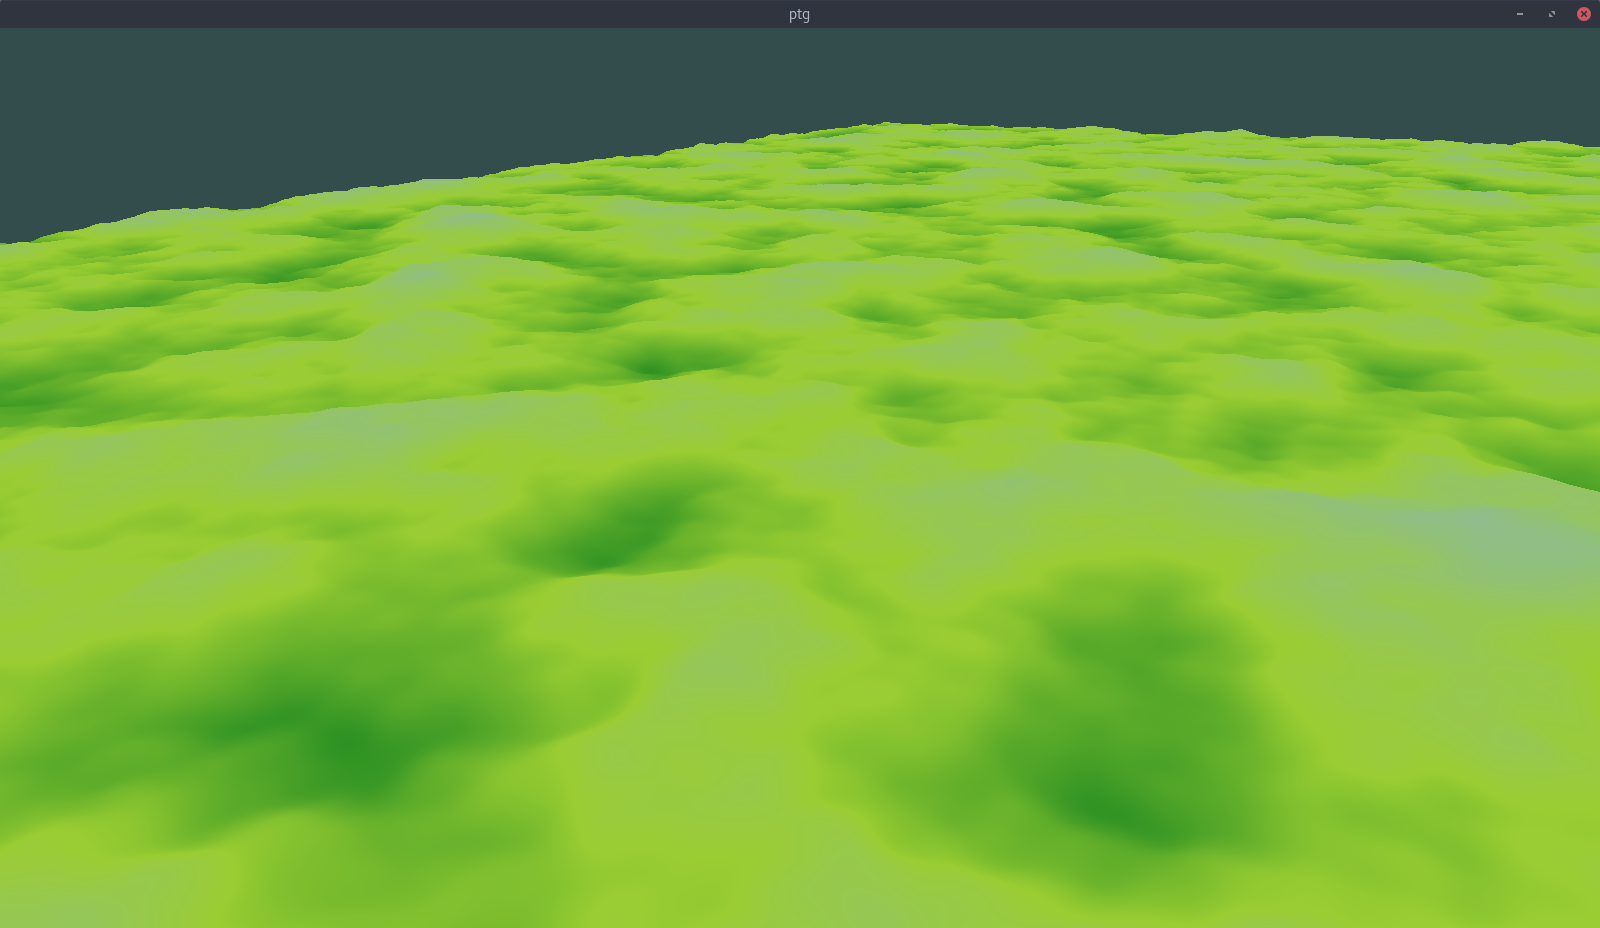
\includegraphics[width=.9\textwidth]{img/biomas/bssPlains.png}
        \caption{Bioma: Planícies.}
        \label{fig:img_biomas_bssPlains}
    \end{figure}
    
    
\end{frame}

\begin{frame}{Biomas}
    \begin{figure}[H]
        \centering
        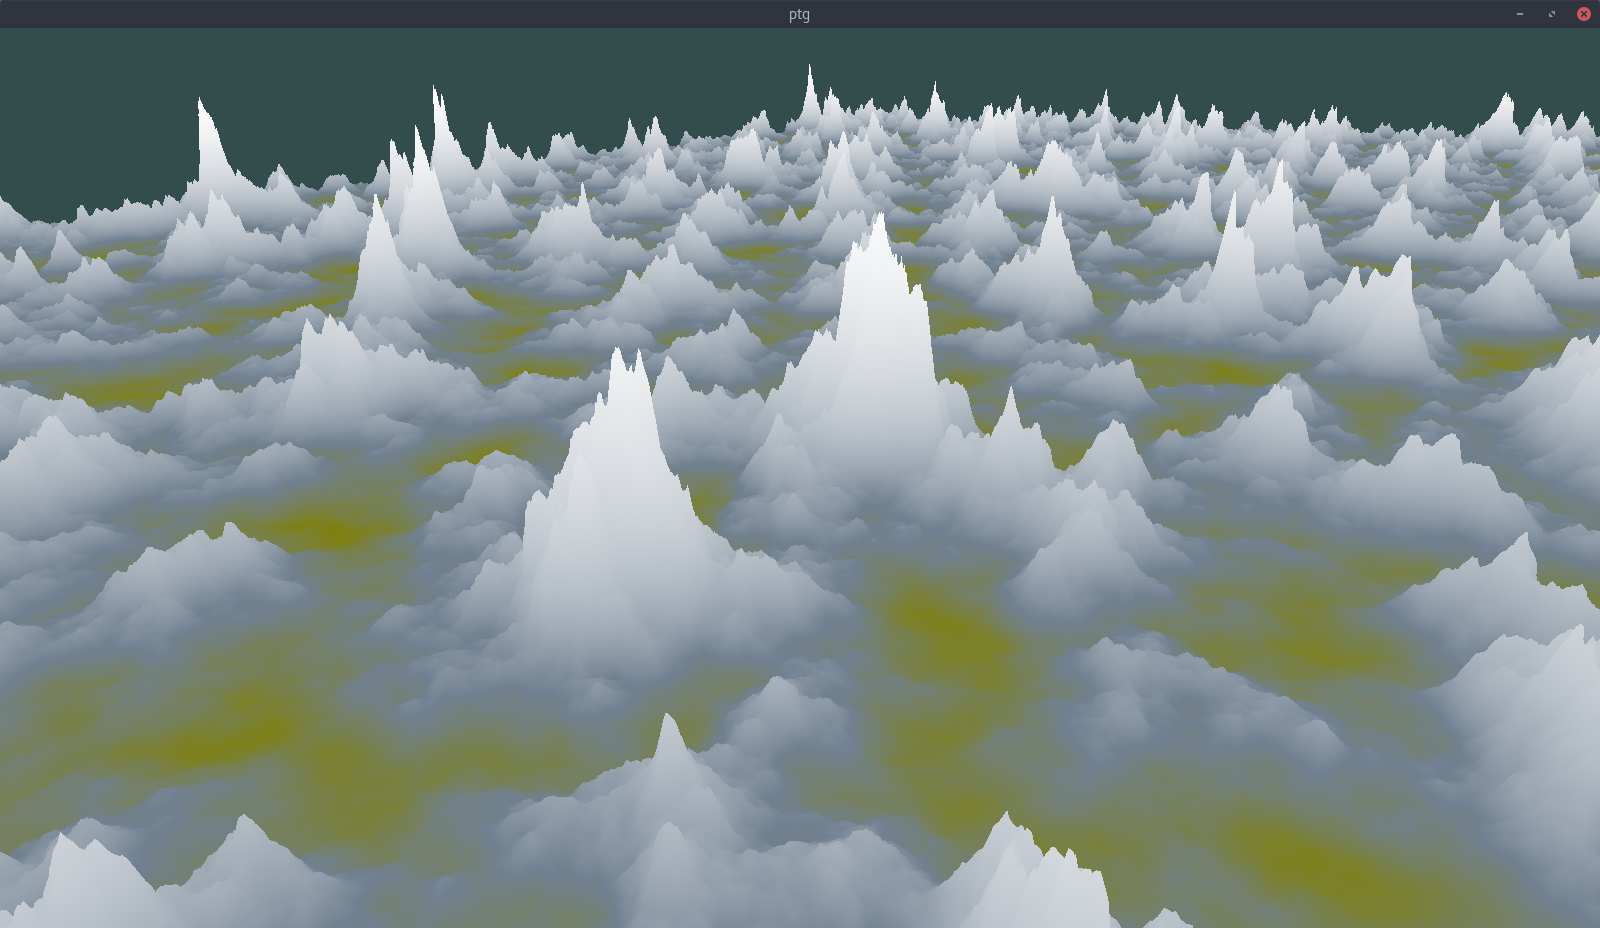
\includegraphics[width=.9\textwidth]{img/biomas/bssMontains.png}
        \caption{Bioma: Montanhas.}
        \label{fig:img_biomas_bssMontains}
    \end{figure}
    
    
\end{frame}

\begin{frame}{Biomas}
    \begin{figure}[H]
        \centering
        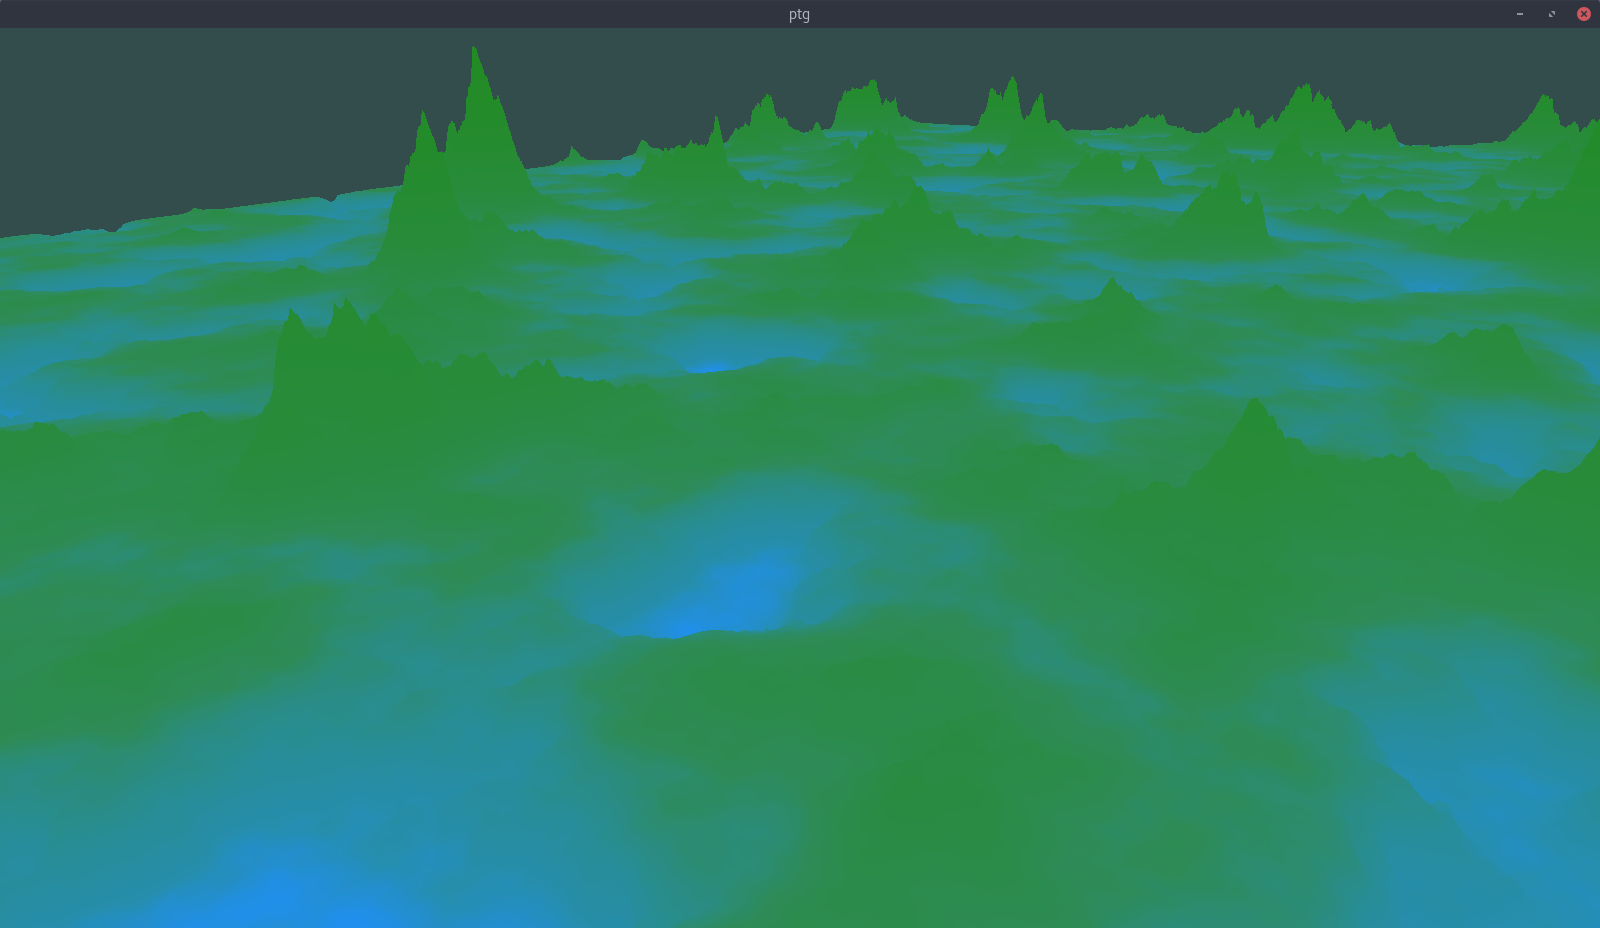
\includegraphics[width=.9\textwidth]{img/biomas/bssValley.png}
        \caption{Bioma: Vales.}
        \label{fig:img_biomas_bssValley}
    \end{figure}
    
    
\end{frame}

\begin{frame}{Biomas}
    \begin{figure}[H]
        \centering
        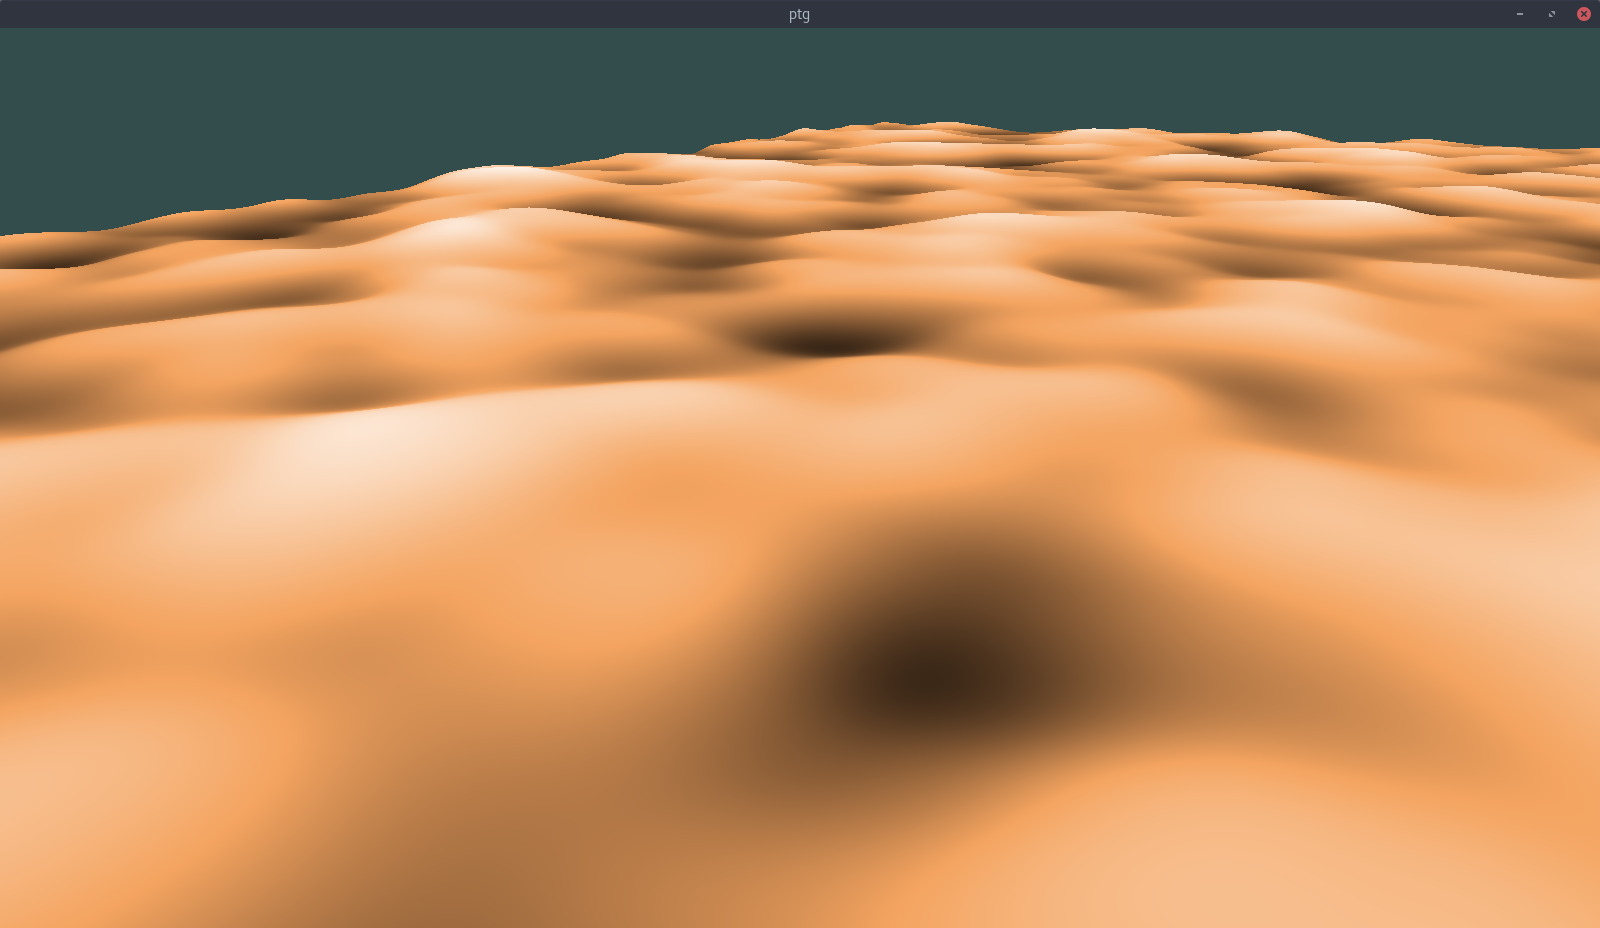
\includegraphics[width=.9\textwidth]{img/biomas/bssDesert.png}
        \caption{Bioma: Deserto.}
        \label{fig:img_biomas_bssDesert}
    \end{figure}
    
    
\end{frame}

\begin{frame}{Biomas}
    \begin{figure}[H]
        \centering
        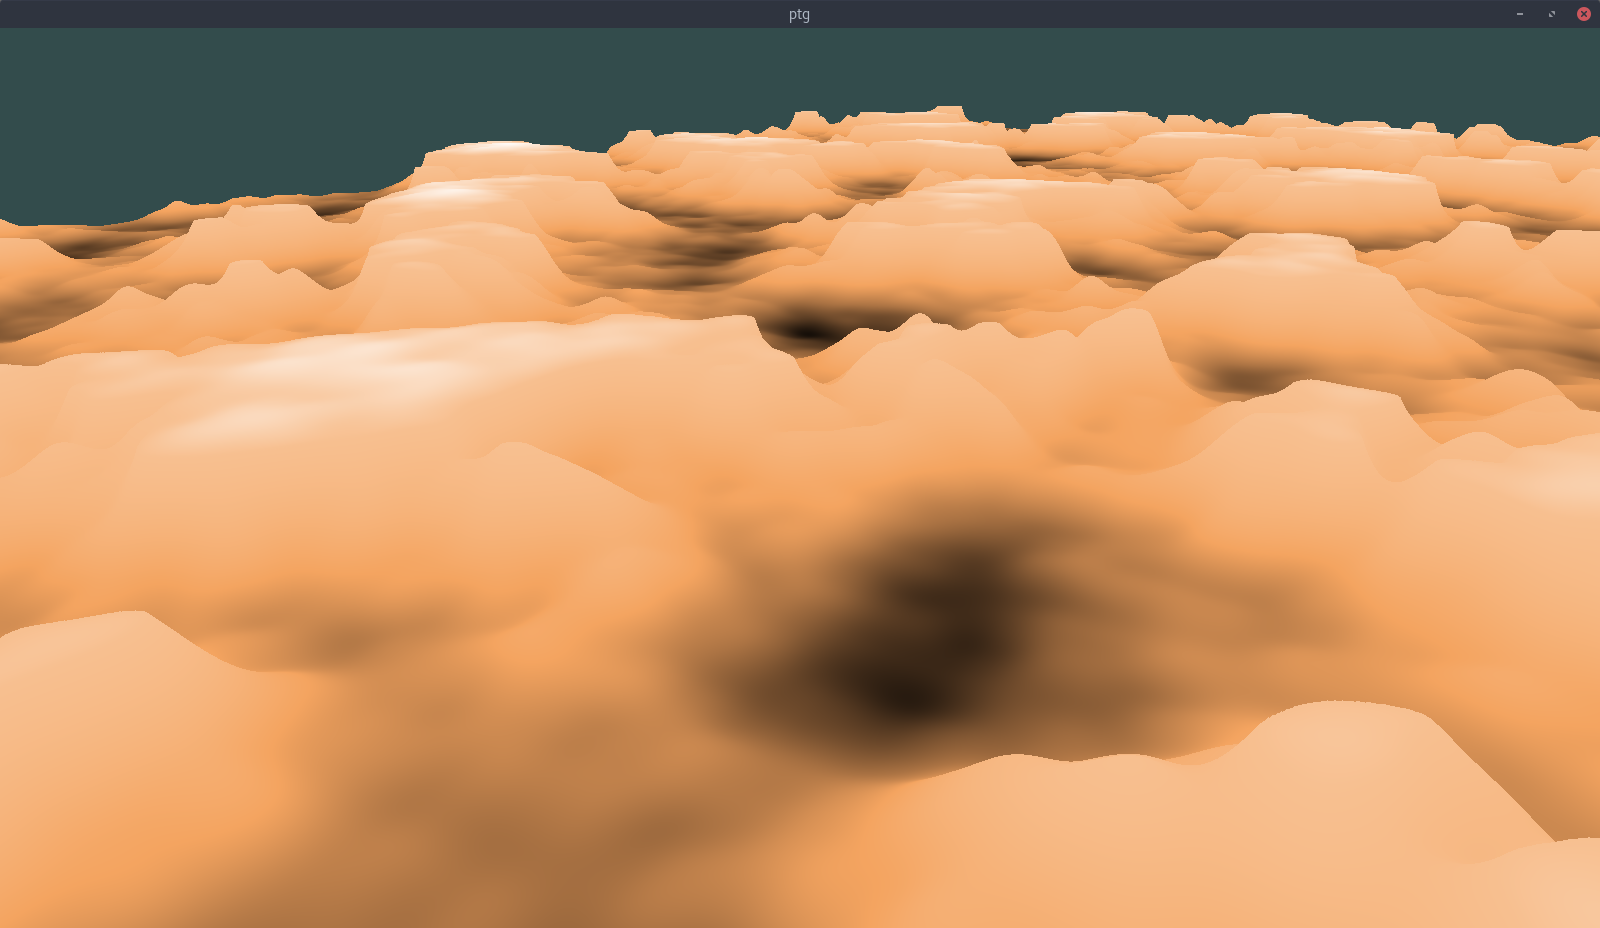
\includegraphics[width=.9\textwidth]{img/biomas/bssCanyons.png}
        \caption{Bioma: Cânyons.}
        \label{fig:img_biomas_bssCanyons}
    \end{figure}
    
    
\end{frame}
\begin{frame}{Malha de Biomas}
    \begin{itemize} \setlength\itemsep{1em}
        \item As regiões de biomas tem áreas quadradas de lado $b$;
    \end{itemize}
\end{frame}

\begin{frame}{Regiões dos Biomas}
    \begin{figure}[H]
        \centering
        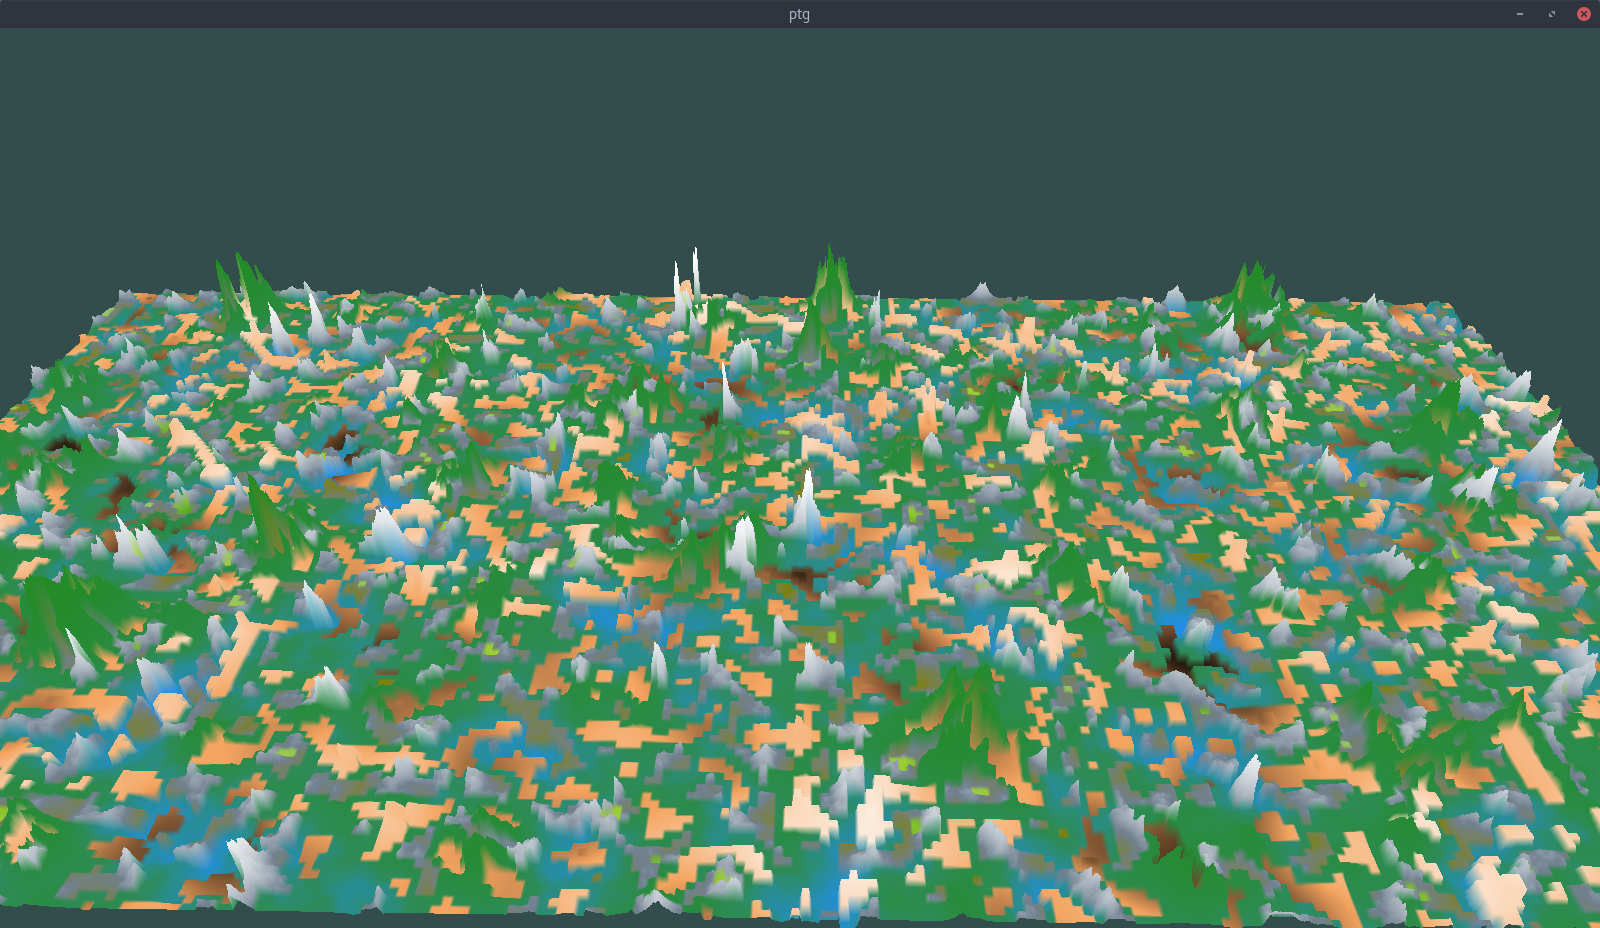
\includegraphics[width=.9\textwidth]{img/re2bfb/b/16f4.png}
        \caption{Regiões com $b = 16$.}
        \label{fig:img_re2bfb_b_16f4}
    \end{figure}
    
    
\end{frame}

\begin{frame}{Malha de Biomas}
    \begin{figure}[H]
        \centering
        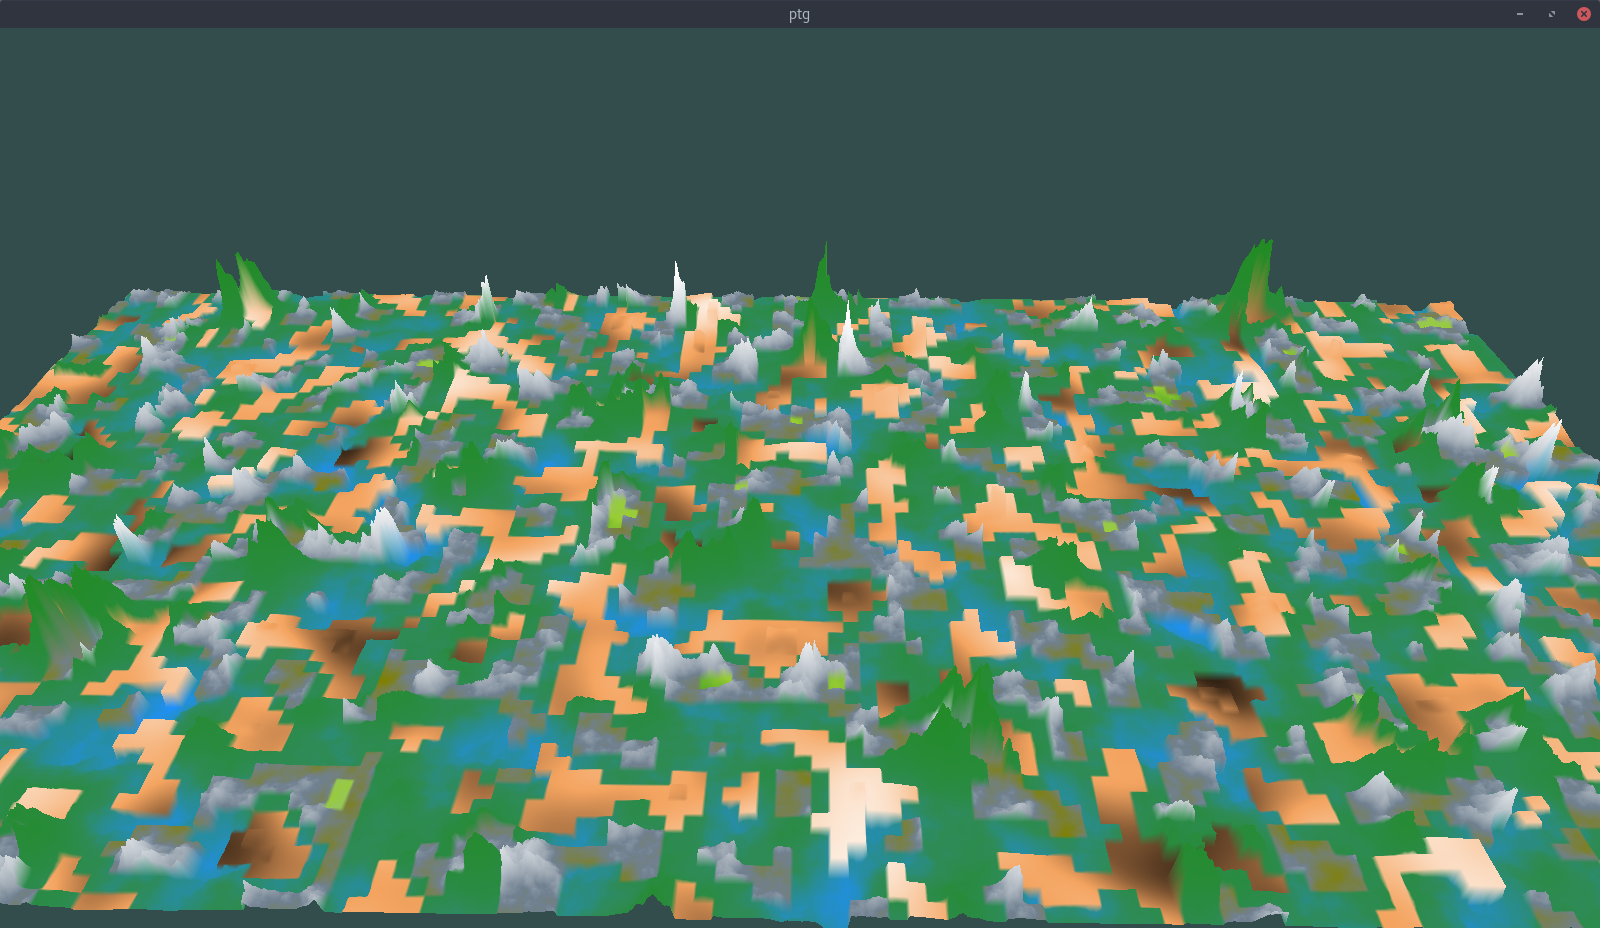
\includegraphics[width=.9\textwidth]{img/re2bfb/b/32f4.png}
        \caption{Regiões com $b = 32$.}
        \label{fig:img_re2bfb_b_32f4}
    \end{figure}
    
    
\end{frame}

\begin{frame}{Malha de Biomas}
    \begin{figure}[H]
        \centering
        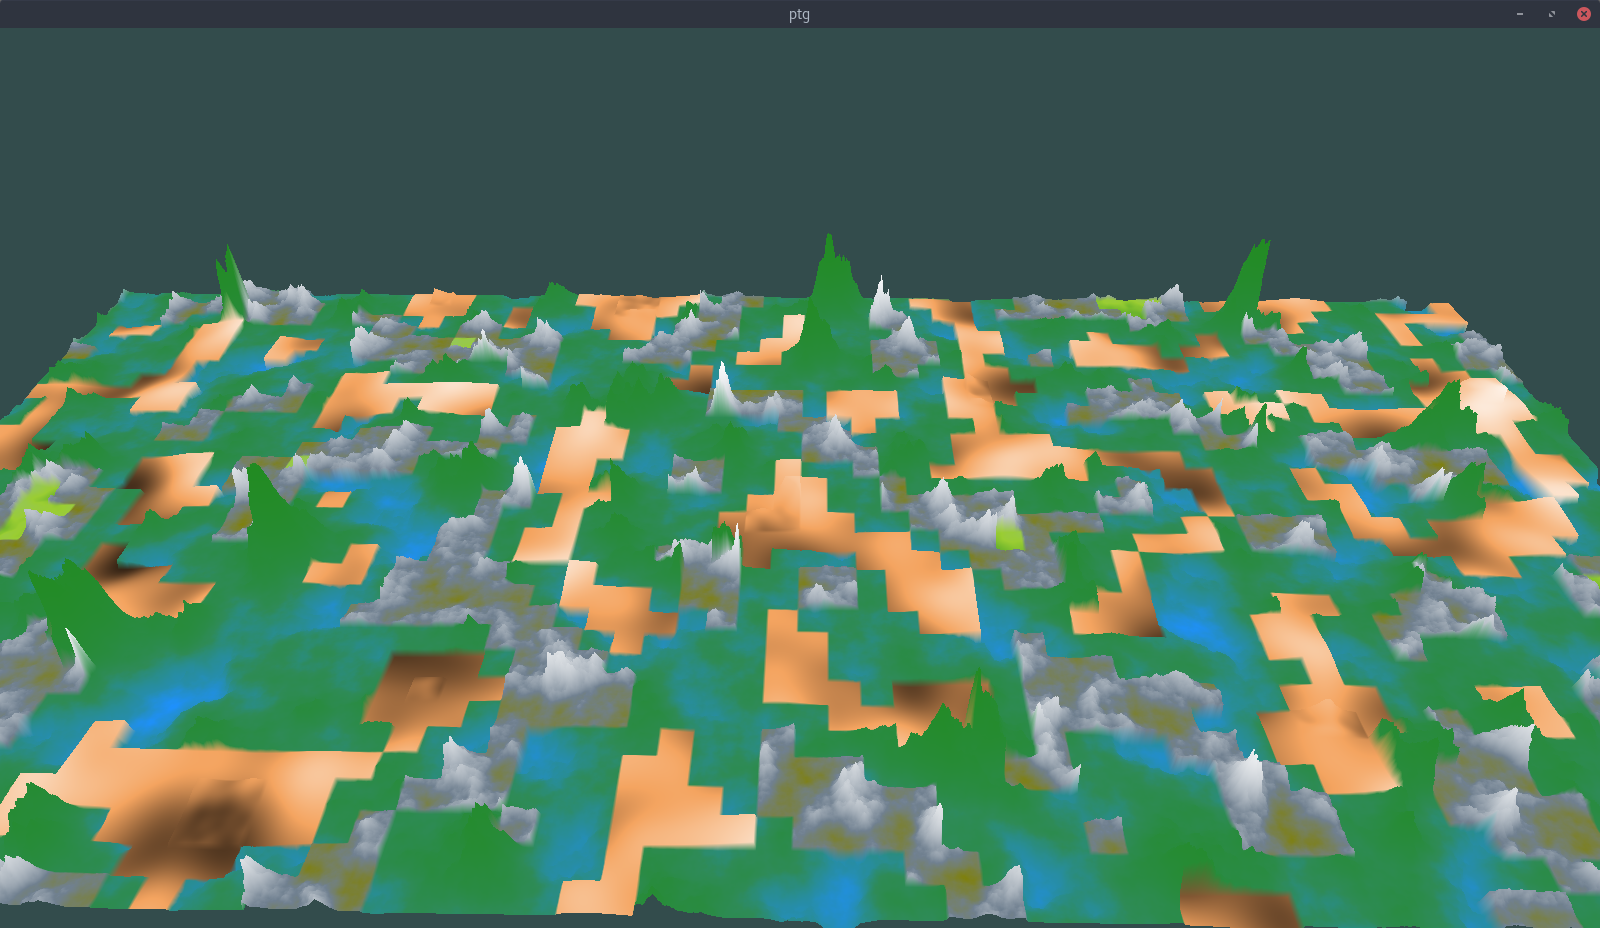
\includegraphics[width=.9\textwidth]{img/re2bfb/b/64f4.png}
        \caption{Regiões com $b = 64$.}
        \label{fig:img_re2bfb_b_64f4}
    \end{figure}
    
    
\end{frame}

\begin{frame}{Malha de Biomas}
    \begin{figure}[H]
        \centering
        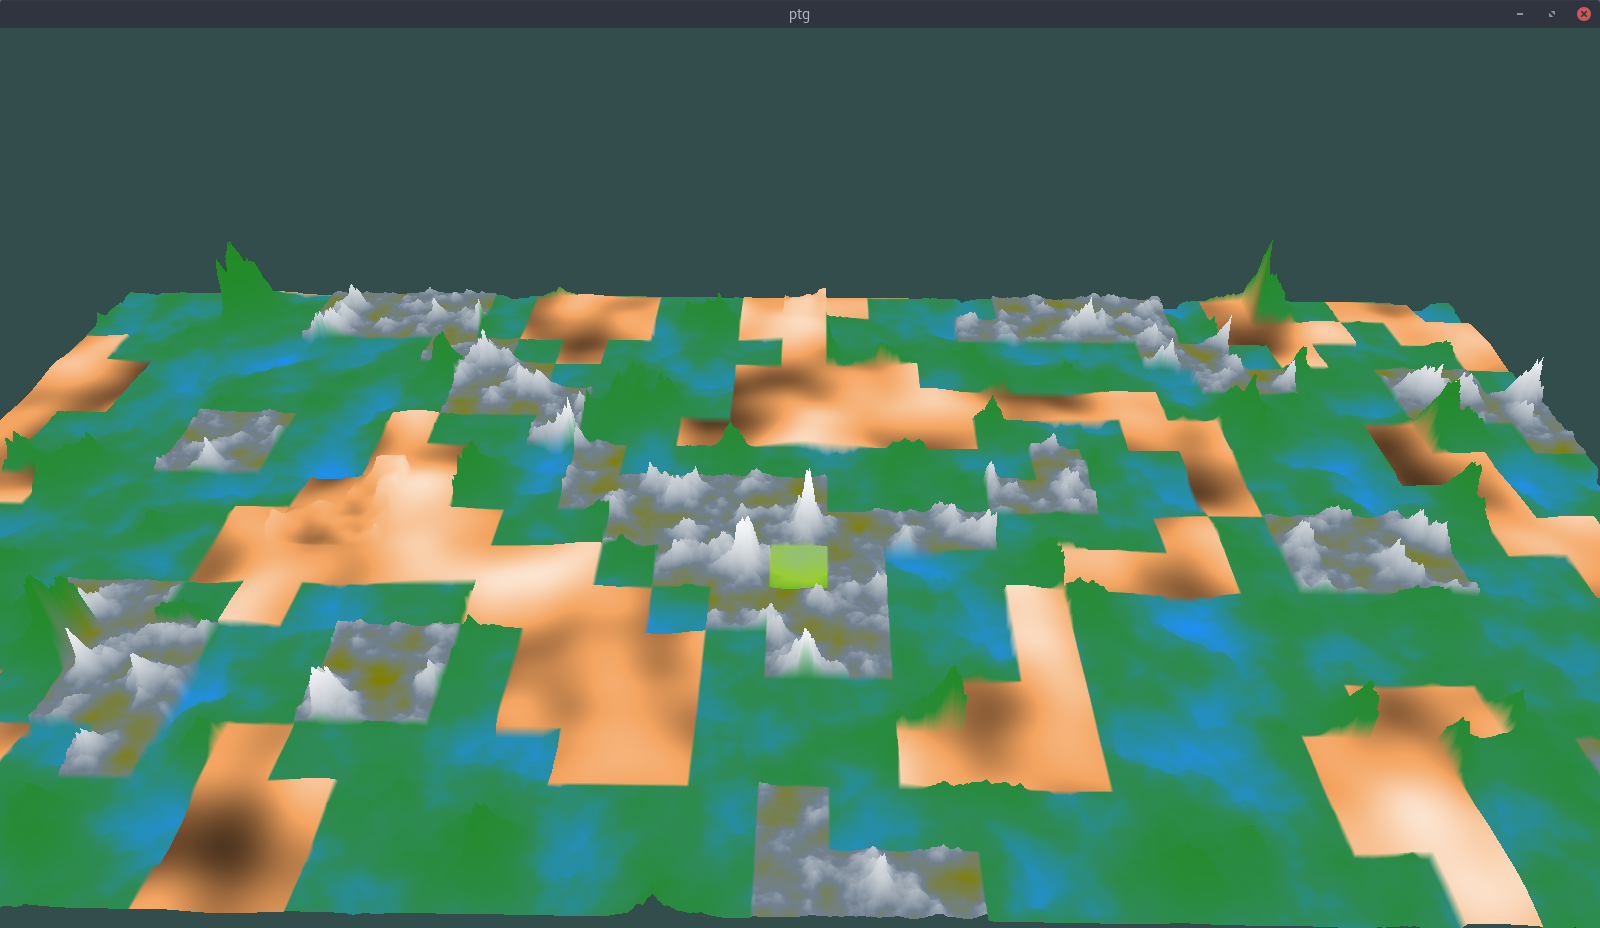
\includegraphics[width=.9\textwidth]{img/re2bfb/b/128f4.png}
        \caption{Regiões com $b = 128$.}
        \label{fig:img_re2bfb_b_128f4}
    \end{figure}
    
    
\end{frame}

\begin{frame}{Malha de Biomas}
    \begin{figure}[H]
        \centering
        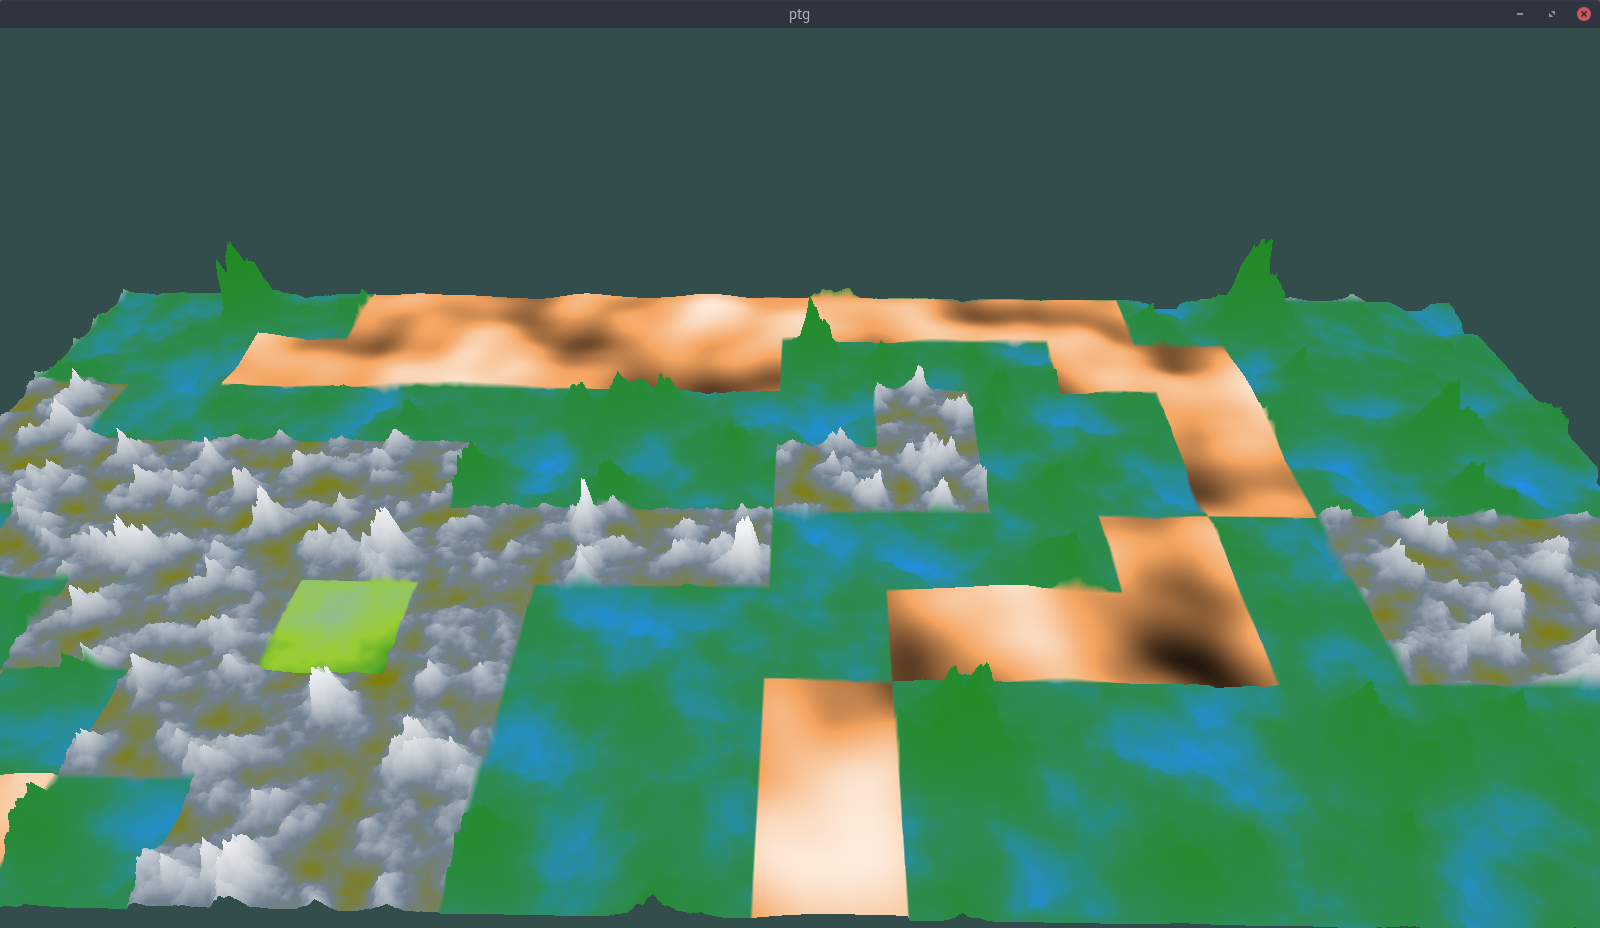
\includegraphics[width=.9\textwidth]{img/re2bfb/b/256f4.png}
        \caption{Regiões com $b = 256$.}
        \label{fig:img_re2bfb_b_256f4}
    \end{figure}
    
    
\end{frame}

\begin{frame}{Malha de Biomas}
    \begin{figure}[H]
        \centering
        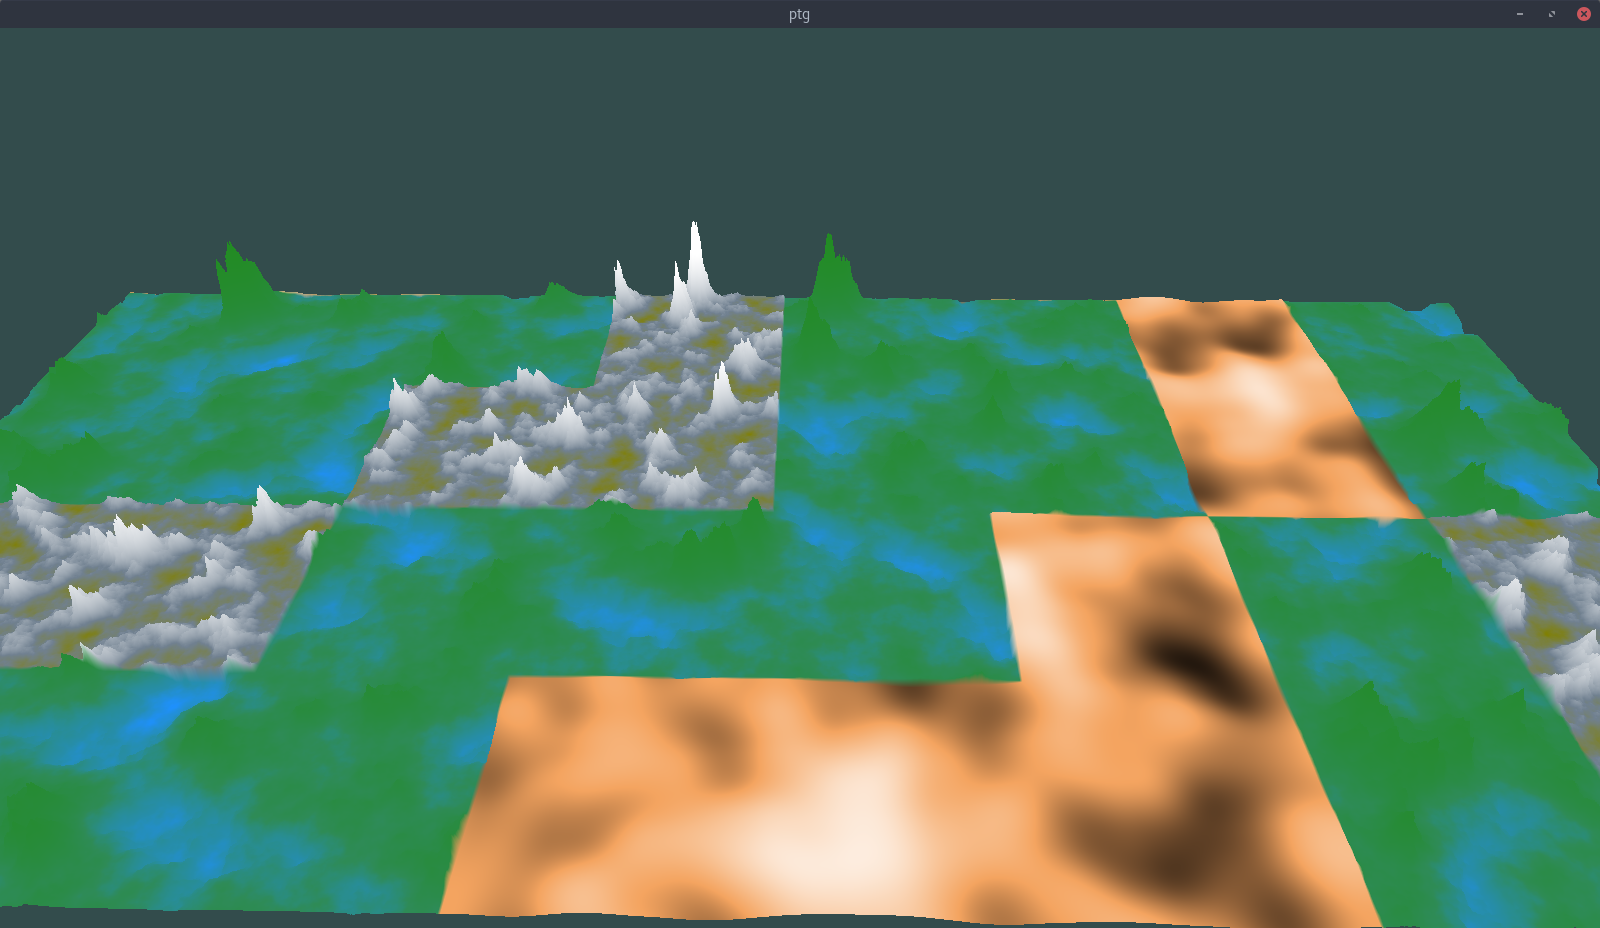
\includegraphics[width=.9\textwidth]{img/re2bfb/b/512f4.png}
        \caption{Regiões com $b = 512$.}
        \label{fig:img_re2bfb_b_512f4}
    \end{figure}
    
    
\end{frame}

\begin{frame}{Malha de Biomas}
    \begin{itemize} \setlength\itemsep{1em}
        \item Cada região usa a chave $(dxs, dzs)$ como parâmetro de ruído para definir seu bioma
        \item A frequência com que mudam os biomas ao longo da malha é $1/fb$
        \item Vantagem de usar ruído para distribuir os biomas
        \begin{figure}[H]
            \centering
            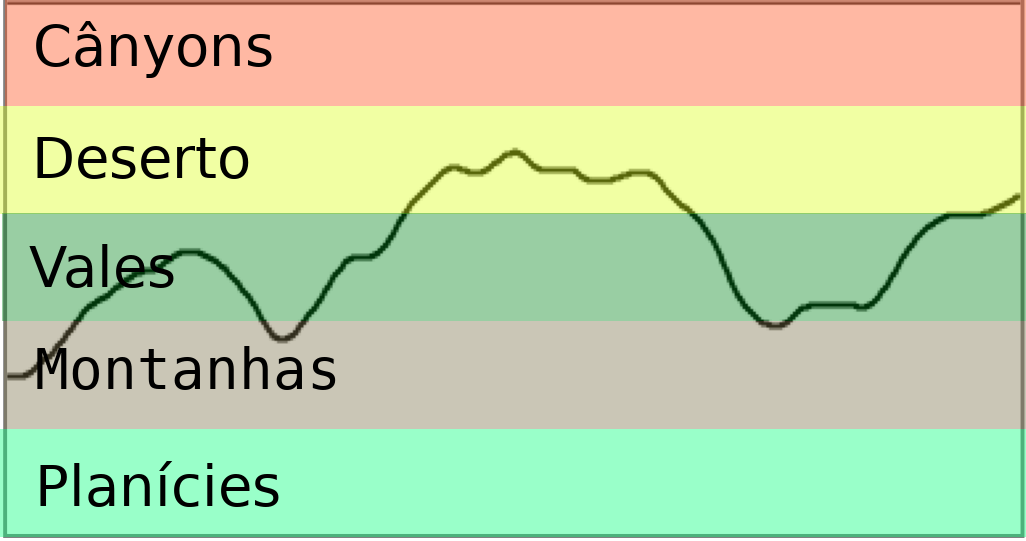
\includegraphics[width=.6\textwidth]{img/re2bfb/distnoise.png}
            \caption{Distribuições de biomas, ruído ao fundo \cite{shiffman2012nature}.}
            \label{fig:img_re2bfb_distnoise}
        \end{figure}
    \end{itemize}
\end{frame}

\begin{frame}{Malha de Biomas}
    \begin{figure}[H]
        \centering
        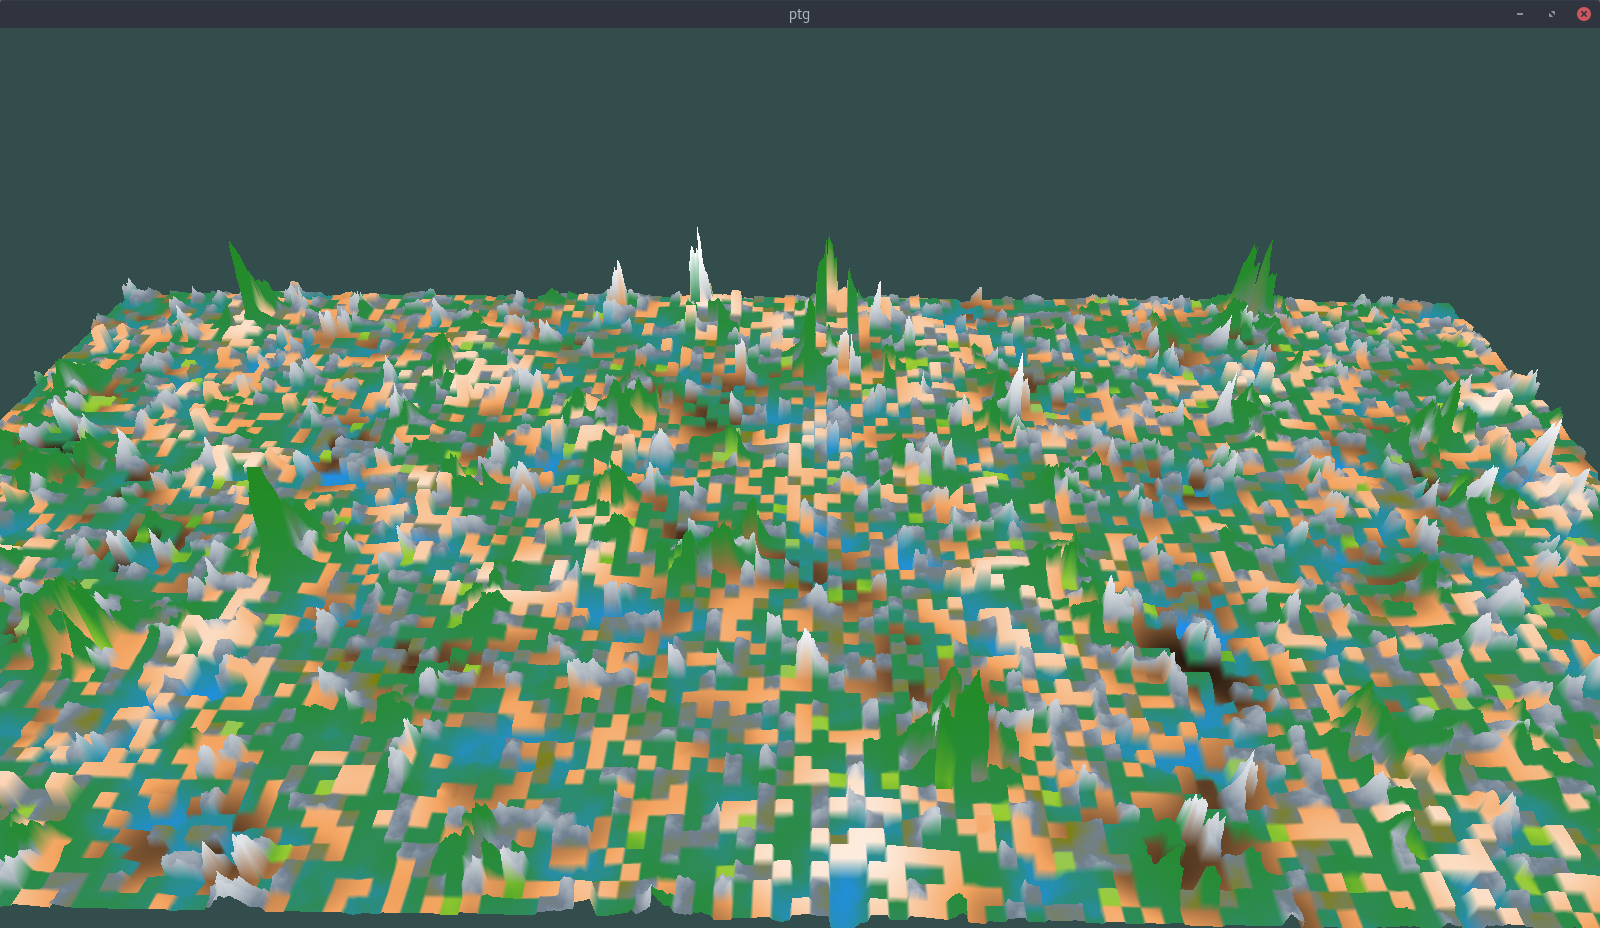
\includegraphics[width=.9\textwidth]{img/re2bfb/fb/05b32.png}
        \caption{Regiões com $b = 32$ e $fb = 0.5$.}
        \label{fig:img_re2bfb_fb_05b32}
    \end{figure}
    
    
\end{frame}

\begin{frame}{Malha de Biomas}
    \begin{figure}[H]
        \centering
        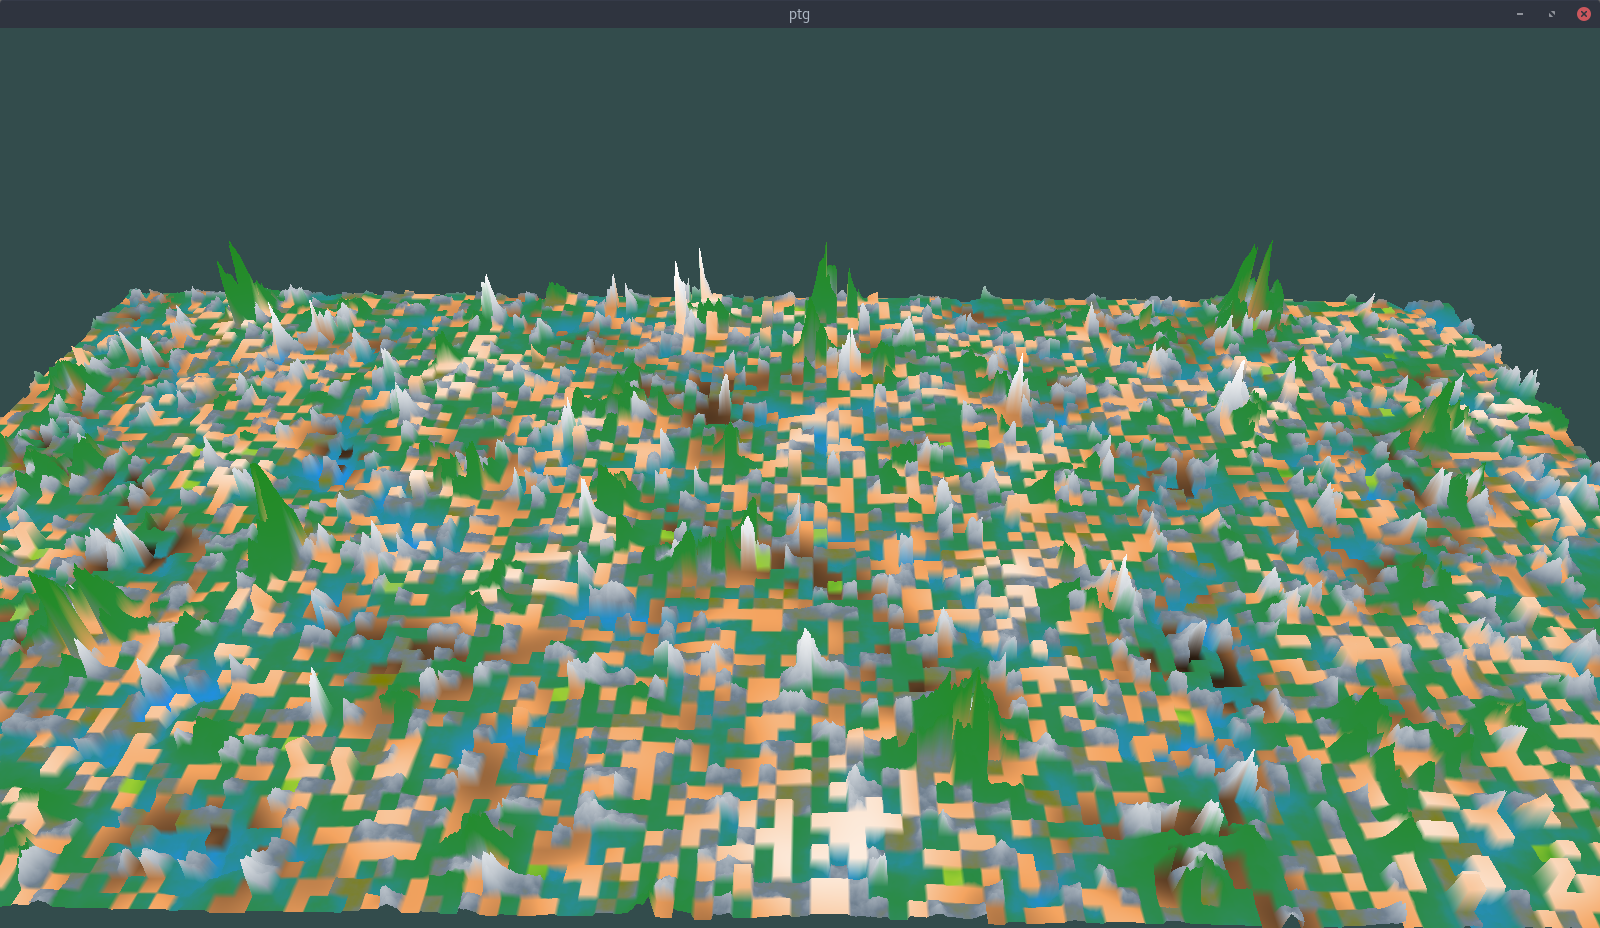
\includegraphics[width=.9\textwidth]{img/re2bfb/fb/1b32.png}
        \caption{Regiões com $b = 32$ e $fb = 1$.}
        \label{fig:img_re2bfb_fb_1b32}
    \end{figure}
    
    
\end{frame}

\begin{frame}{Malha de Biomas}
    \begin{figure}[H]
        \centering
        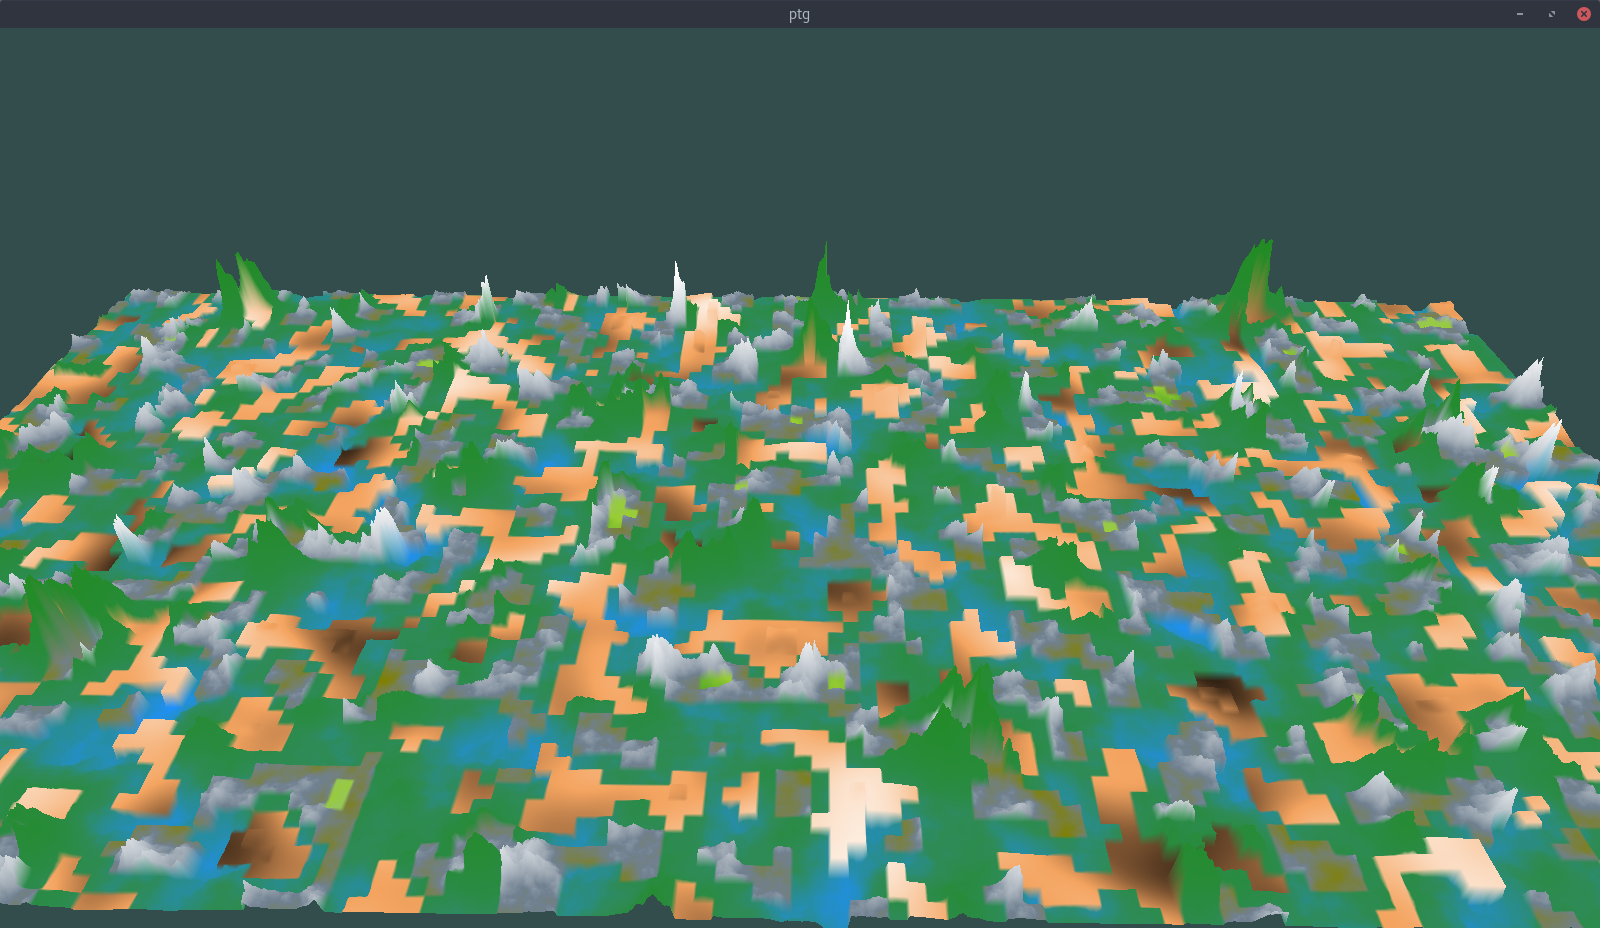
\includegraphics[width=.9\textwidth]{img/re2bfb/fb/4b32.png}
        \caption{Regiões com $b = 32$ e $fb = 4$.}
        \label{fig:img_re2bfb_fb_4b32}
    \end{figure}
    
    
\end{frame}

\begin{frame}{Malha de Biomas}
    \begin{figure}[H]
        \centering
        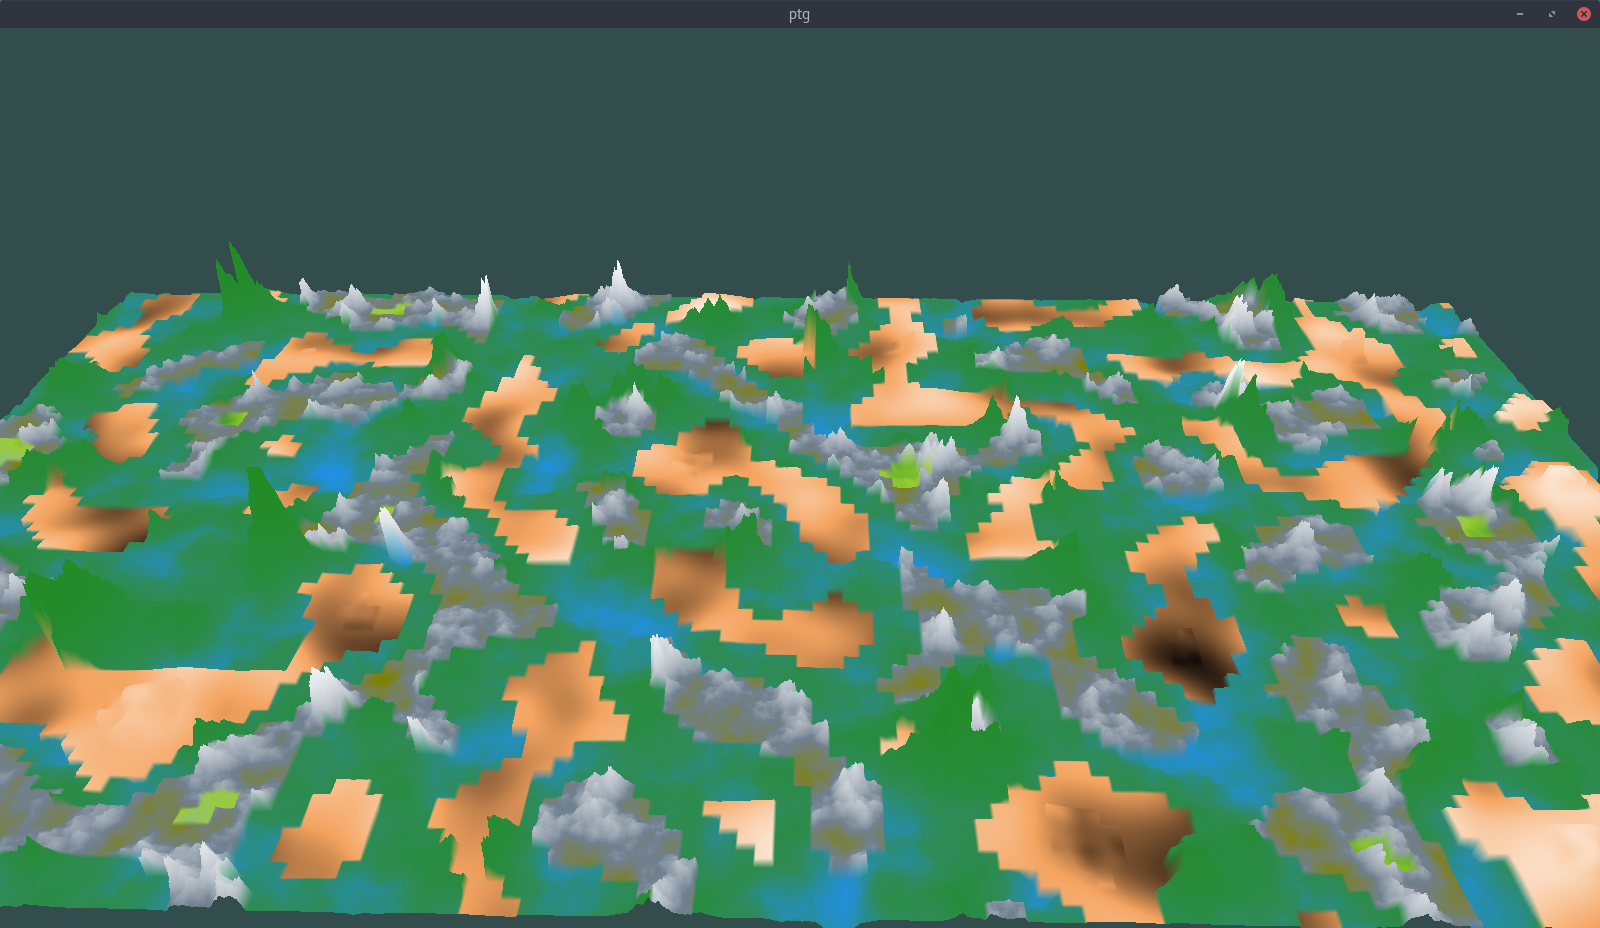
\includegraphics[width=.9\textwidth]{img/re2bfb/fb/8b32.png}
        \caption{Regiões com $b = 32$ e $fb = 8$.}
        \label{fig:img_re2bfb_fb_8b32}
    \end{figure}
    
    
\end{frame}

\begin{frame}{Malha de Biomas}
    \begin{figure}[H]
        \centering
        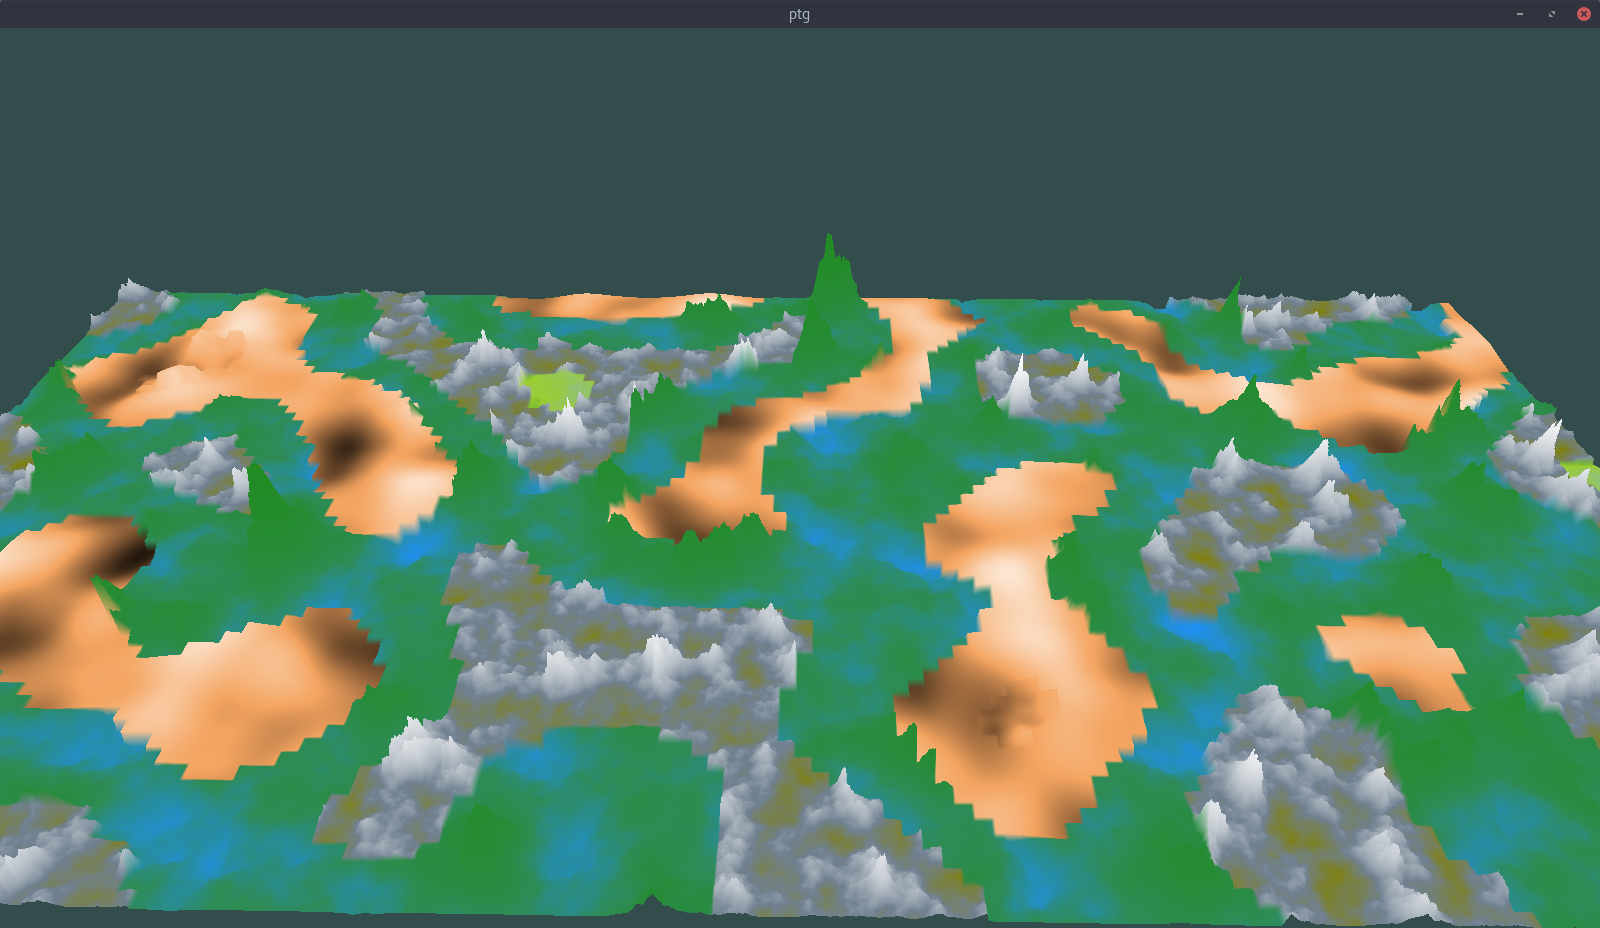
\includegraphics[width=.9\textwidth]{img/re2bfb/fb/16b32.png}
        \caption{Regiões com $b = 32$ e $fb = 16$.}
        \label{fig:img_re2bfb_fb_16b32}
    \end{figure}
    
    
\end{frame}

\begin{frame}{Malha de Biomas}
    \begin{figure}[H]
        \centering
        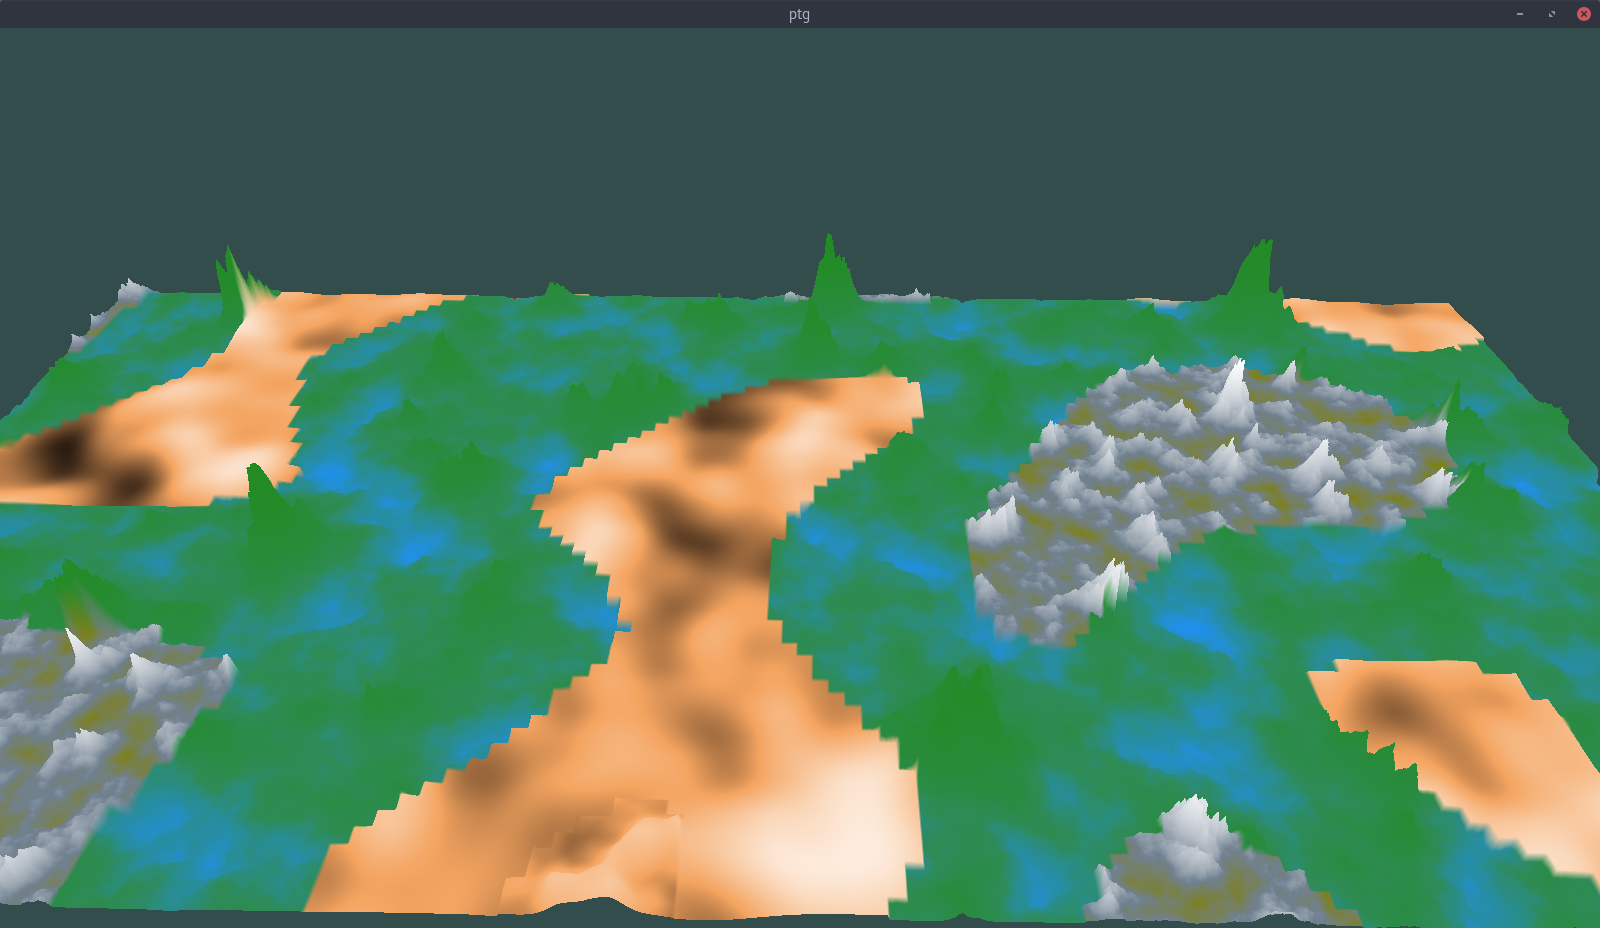
\includegraphics[width=.9\textwidth]{img/re2bfb/fb/32b32.png}
        \caption{Regiões com $b = 32$ e $fb = 32$.}
        \label{fig:img_re2bfb_fb_32b32}
    \end{figure}
    
    
\end{frame}

\begin{frame}{Malha de Biomas}
    \begin{figure}[H]
        \centering
        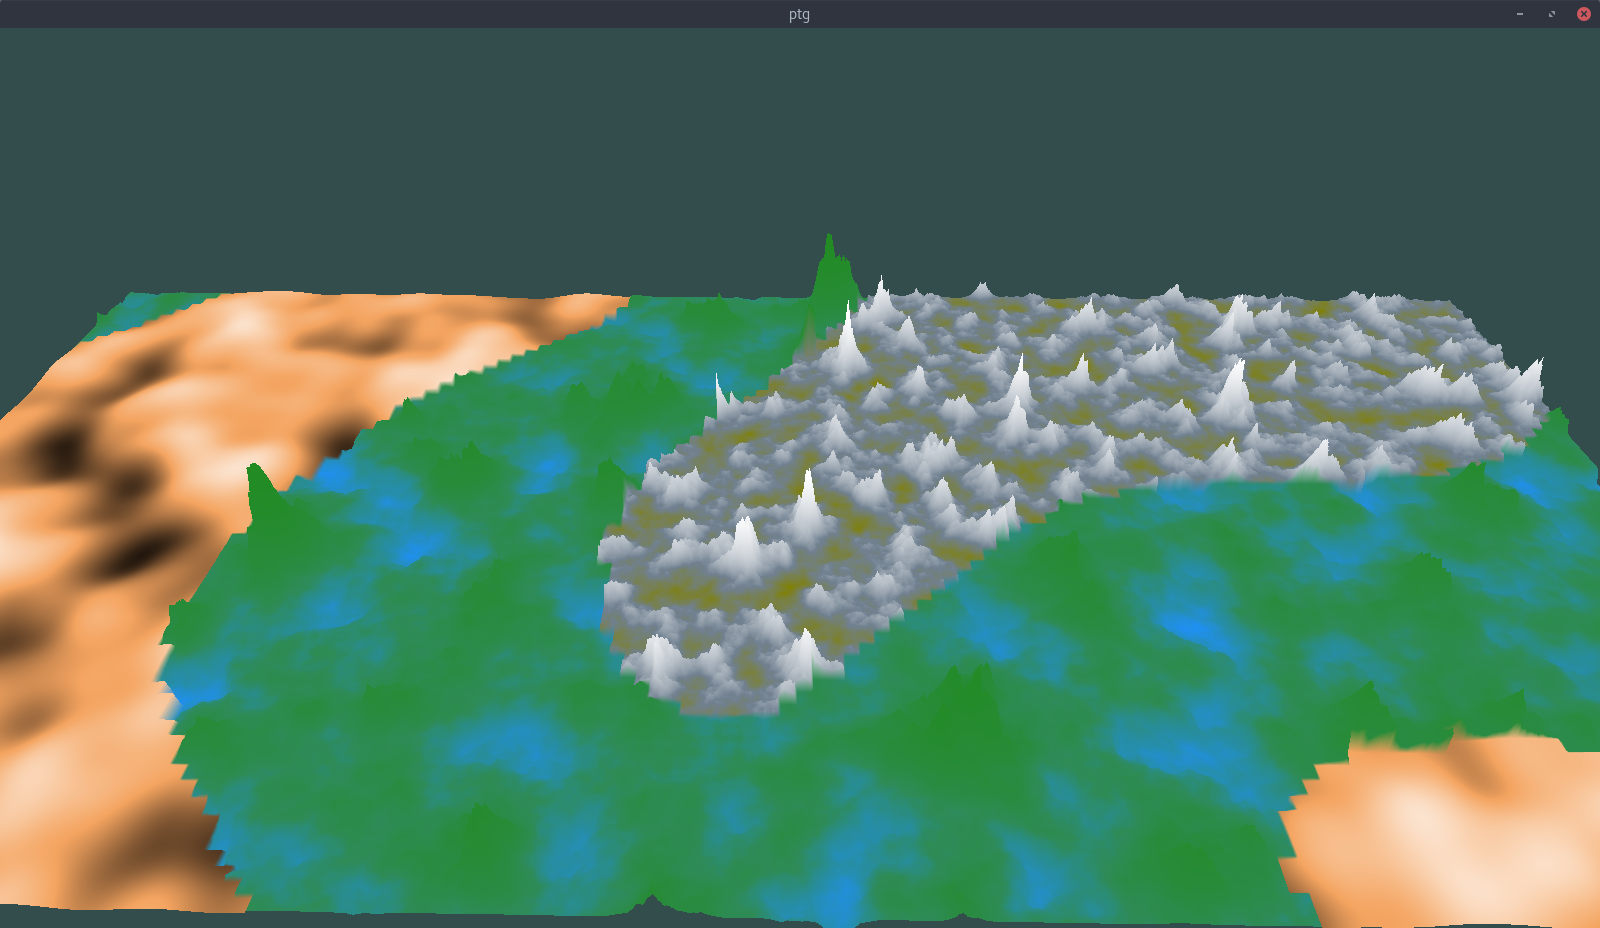
\includegraphics[width=.9\textwidth]{img/re2bfb/fb/64b32.png}
        \caption{Regiões com $b = 32$ e $fb = 64$.}
        \label{fig:img_re2bfb_fb_64b32}
    \end{figure}
    
    
\end{frame}
%pdflatex apresentacao.tex 
%bibtex apresentacao.aux
%pdflatex apresentacao.tex 
%pdflatex apresentacao.tex 

\begin{frame}{Ruído de Perlin}
    \begin{itemize}\setlength\itemsep{1em}
        \item Falar sobre ruído de  \cite{perlin2002improving} aqui =D    
    \end{itemize}
    \begin{figure}[H]
        \centering
        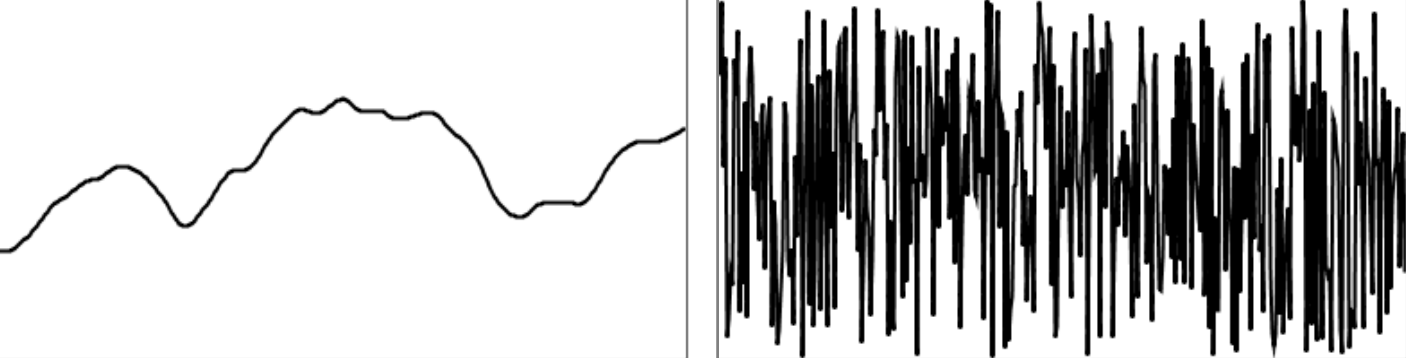
\includegraphics[width=.75\textwidth]{img/randomAndNoise}
        \caption{Da esquerda: Função de ruído e função que gera números aleatórios. Por \cite{shiffman2012nature}}
        \label{fig:randomAndNoise}
    \end{figure}
    
\end{frame}

\begin{frame}{Ruído de Perlin}
    \begin{itemize}\setlength\itemsep{1em}
        \item Falar sobre ruído de  
    \end{itemize}
    \begin{figure}[H]
        \centering
        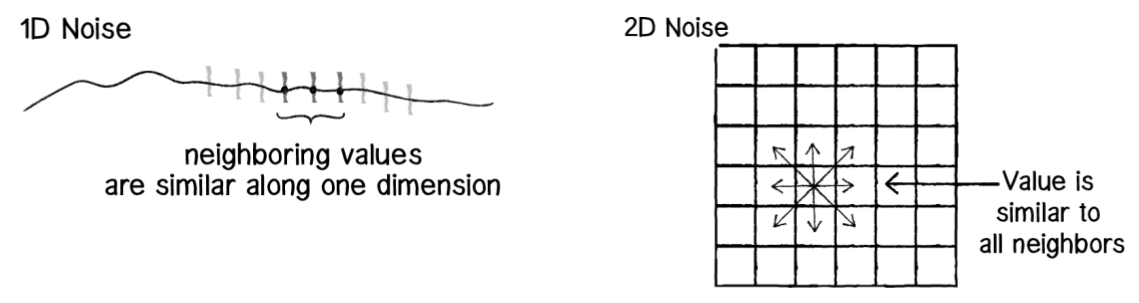
\includegraphics[width=.75\textwidth]{img/1dto2dnoise}
        \caption{À esquerda relação entre pontos unidimensionais, à direita bidimensionais. Por \cite{shiffman2012nature}}
        \label{fig:1dto2dnoise}
    \end{figure}
    
\end{frame}



\begin{frame}{Ruído de Perlin}
    
    \begin{figure}
        \centering
        \begin{subfigure}[b]{0.6\textwidth}
            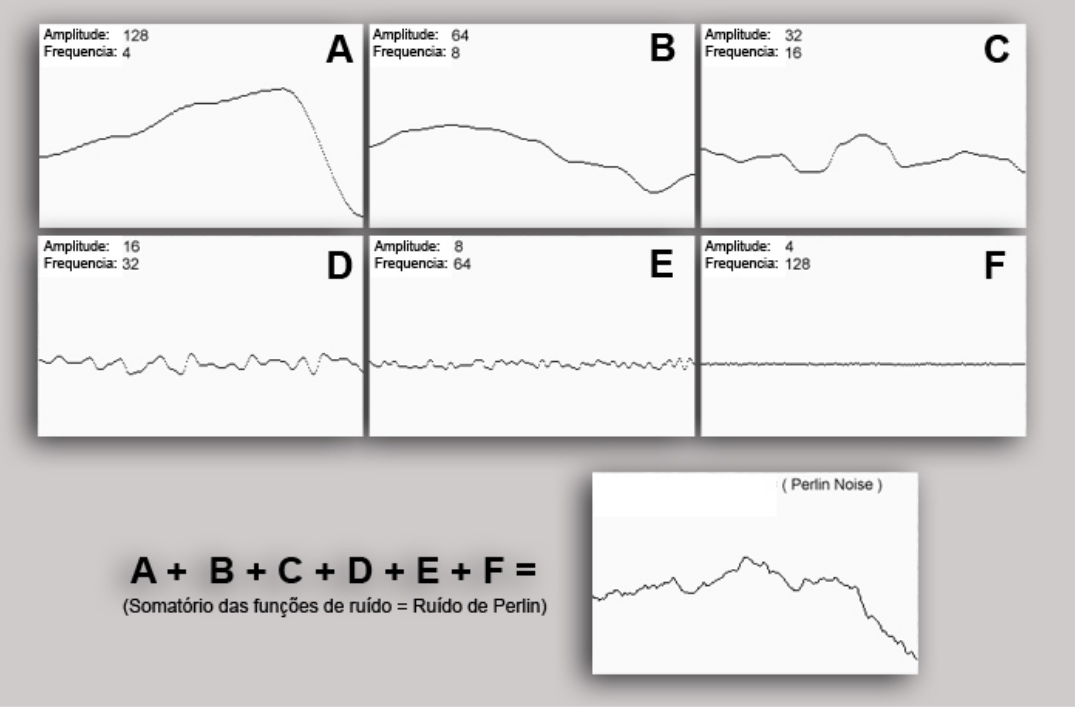
\includegraphics[width=\textwidth]{img/perlin1d}
            \caption{Ruído de Perlin com uma dimensão}
            \label{fig:perlin1d}
        \end{subfigure}
        ~ %add desired spacing between images, e. g. ~, \quad, \qquad, \hfill etc. 
          %(or a blank line to force the subfigure onto a new line)
        \begin{subfigure}[b]{0.35\textwidth}
            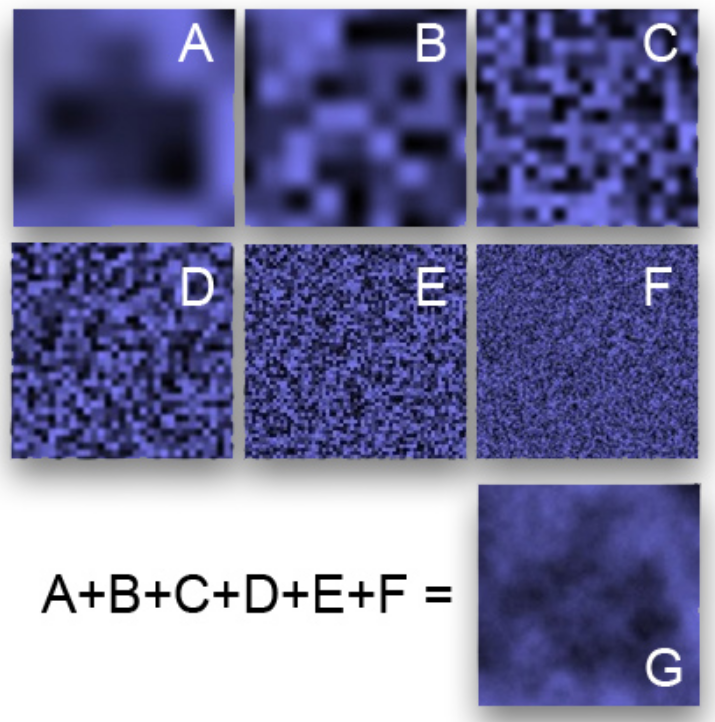
\includegraphics[width=\textwidth]{img/perlin2d}
            \caption{Ruído de Perlin com duas dimensões}
            \label{fig:perlin2d}
        \end{subfigure}
        ~ %add desired spacing between images, e. g. ~, \quad, \qquad, \hfill etc. 
        %(or a blank line to force the subfigure onto a new line)
        \caption{Perlin para uma e duas dimensões. Por \cite{elias2000perlin}}
        \label{fig:perlin1d2d}
    \end{figure}
    
\end{frame}


\begin{frame}{Mapas de Altura}
    
    \begin{figure}[H]
        \centering
        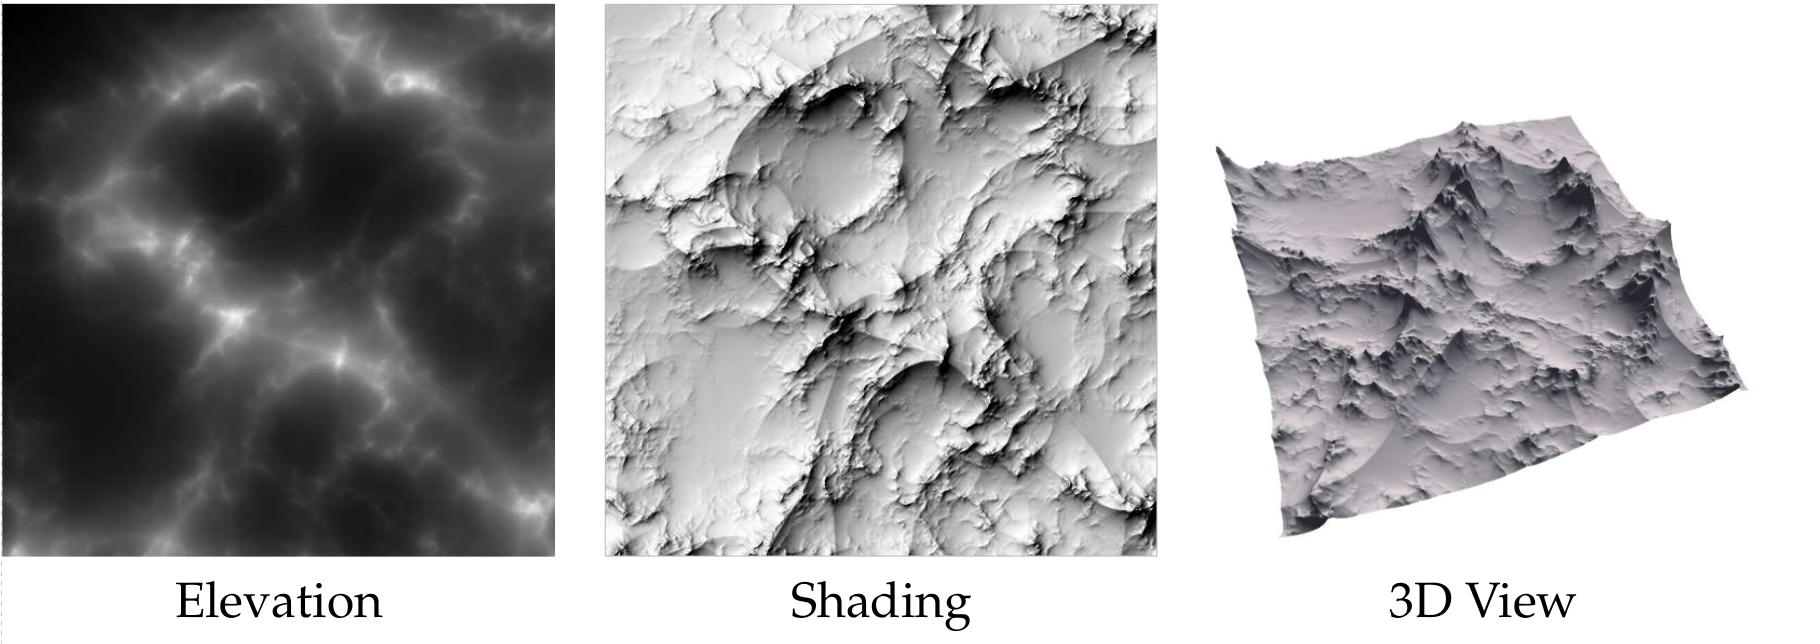
\includegraphics[width=.75\textwidth]{img/hmap}
        \caption{Mapa de altura em diferentes perspectivas. Por \cite{dachsbacher2006interactive}}
        \label{fig:hmap}
    \end{figure}
\end{frame}
\chapter{Metodologia}
Nesta seção veremos a metodologia do trabalho desde a busca por fontes e trabalhos
relacionados até a analise de resultados.

Começando pela leitura de trabalhos relacionados, os primeiros trabalhos lidos
foram recomendados por professores, a partir destes trabalhos li algumas de suas
referências mais relevantes, os mesmos continham outras citações relevantes, e
assim por diante, dessa maneira, tenho em mãos uma "árvore" de citações,
para preencher algumas lacunas e reforçar alguns argumentos foram necessárias
mais buscas de artigos e trabalhos.

%Selecionar maneira de separar regiões;
A primeira etapa da implementação é escolher a maneira em que regiões serão
separadas, um bioma vai pertencer a um conjunto de regiões, as opções
pré-selecionadas são: \textit{Triangle strip}, malha de quadrados e diagrama de
voronoi. Cada uma delas tem sua vantagem, diagrama de voronoi constrói fronteiras
mais naturais, as outras técnicas tem implementação mais fácil, menor custo
computacional e geram a possibilidade de trabalhar com mapas pseudo infinitos.
Então serão implementadas as três e feitas comparações sobre elas para decidir
qual a melhor opção. A decisão será tomada...
NÃO FAÇO A MENOR IDEIA DE COMO ESSA DECISÃO VAI SER FEITA.

%Selecionar biomas, e as características dos mesmos a ser representadas;
Próxima etapa é a escolha de biomas e suas características a serem geradas pelo%estou repetindo de mais a palavra caracteristica, preciso dar um jeito nisso
algoritmo, a principio a escolha será feita por características fáceis de
implementar, biomas com características mais distintas, para ser visualmente
mais fácil de distinguir regiões de um e outro.%Construir algoritmo para manipular ruído de Perlin e gerar características selecionadas do bioma;
E como já visto no trabalho de \cite{carli2012canion}, podemos manipular o ruído
de Perlin para imitar as características de alguns padrões da natureza, então, 
o mesmo será feito para os biomas selecionados.

%Implementar fronteiras contínuas entre biomas;
Caso não tratado, as fronteiras em biomas podem e provavelmente serão
descontinuas, tendo uma mudança brusca de altura nas fronteiras e deixando o
cenário sem sentido, então nesta etapa será analisadas as possibilidades para
correção da descontinuidade e implementar a mesma.

%Comparar resultado com cenários de jogos e Comparar resultados com a natureza.


\setbeamertemplate{footline}{
	\color{white}
     \\
    }

\begin{frame}{Referências} % allowframebreaks -> Referências grandes
   \bibliography{referencias}
   \bibliographystyle{apalike}
\end{frame}

\begin{frame}
	\maketitle
\end{frame}

%% Coloquei o  livro em  anotacoes.bib. Pode incluir  outras referências
%% alí. (AG)

\end{document}
